%%-----------------------------------------------
%% Cargar datos relativos al TFG:
%%%%%%%%%%%%%%%%%%%%%%%%%%%%%%%%%
%% Información para la portada %%
%%%%%%%%%%%%%%%%%%%%%%%%%%%%%%%%%

%% Escribe Nombre y Apellidos del autor del trabajo:
\newcommand{\NombreAutor}{ Carlo Alessandro Cabrera }

%% Escribe el Grado: 
\newcommand{\Grado}{ Ingeniería Informática }

%% Escribe el Título del Trabajo:
\newcommand{\TituloTFG}{ Análisis topológico de trayectorias en baja y alta dimensión } 

%% Escribe Nombre y Apellidos del Tutor del trabajo: 
\newcommand{\NombreTutor}{ Juan Antonio Fernández del Pozo } 

% Escribe el Departamento al que pertenece el Tutor:
\newcommand{\Departamento}{ Departamento de Inteligencia Artificial (DIA) }

% Escribe la fecha de lectura, en formato: Mes - Año
\newcommand{\Fecha}{ JUNIO - 2025 }
%%***********************************************


%%-----------------------------------------------
%% Importar Preámbulo:
% -*-coding: utf-8 -*-
\documentclass[a4paper,11pt,openany]{book}
\usepackage[utf8]{inputenc}
\usepackage[T1]{fontenc}
\usepackage[english,spanish,es-lcroman]{babel}
\usepackage{bookman}
\decimalpoint
\usepackage{graphicx}
\usepackage{amsfonts,amsgen,amsmath,amssymb}
\usepackage[top=3cm, bottom=3cm, right=2.54cm, left=2.54cm]{geometry}
\usepackage{afterpage}
\usepackage{colortbl,longtable}
\usepackage[
  pdftex,
  pdfauthor={\NombreAutor{}},
  pdftitle={Trabajo de Fin de Grado},
  pdfborder={0 0 0}
]{hyperref}
\usepackage{pdfpages}
\usepackage{url}
\usepackage[stable]{footmisc}
\usepackage{parskip} % para separar párrafos con espacio.
\usepackage{lscape}
\usepackage{pgfgantt}

% --- BIBLIOGRAPHY ---
\usepackage[
  backend=biber,
  style=numeric,
  sorting=none
]{biblatex}
\addbibresource{bibliography.bib}
\usepackage{csquotes}
% --- BIBLIOGRAPHY ---

\usepackage{float}
\usepackage{subfigure}

%%-----------------------------------------------
\usepackage{fancyhdr}
\pagestyle{fancy}
\fancyhf{}
\fancyhead[LO]{\leftmark}
\fancyhead[RE]{\rightmark}
\setlength{\headheight}{1.5\headheight}
\cfoot{\thepage}

\addto\captionsspanish{ \renewcommand{\contentsname}
  {Índice general} }
\setcounter{tocdepth}{4}
\setcounter{secnumdepth}{4}

\renewcommand{\chaptermark}[1]{\markboth{\textbf{#1}}{}}
\renewcommand{\sectionmark}[1]{\markright{\textbf{\thesection. #1}}}
\newcommand{\HRule}{\rule{\linewidth}{0.5mm}}
\newcommand{\bigrule}{\titlerule[0.5mm]}

\usepackage{appendix}
\renewcommand{\appendixname}{Anexos}
\renewcommand{\appendixtocname}{Anexos}
\renewcommand{\appendixpagename}{}
%%-----------------------------------------------
%% Páginas en blanco sin cabecera:
%%-----------------------------------------------
\usepackage{dcolumn}
\newcolumntype{.}{D{.}{\esperiod}{-1}}
\makeatletter
\addto\shorthandsspanish{\let\esperiod\es@period@code}

\def\clearpage{
  \ifvmode
  \ifnum \@dbltopnum =\m@ne
  \ifdim \pagetotal <\topskip
  \hbox{}
  \fi
  \fi
  \fi
  \newpage
  \thispagestyle{empty}
  \write\m@ne{}
  \vbox{}
  \penalty -\@Mi
}
\makeatother
%%-----------------------------------------------
%% Estilos código de lenguajes: Consola, C, C++ y Python
%%-----------------------------------------------
\usepackage{color}

\definecolor{gray97}{gray}{.97}
\definecolor{gray75}{gray}{.75}
\definecolor{gray45}{gray}{.45}

\usepackage{listings}
\lstset{ frame=Ltb,
  framerule=0pt,
  aboveskip=0.5cm,
  framextopmargin=3pt,
  framexbottommargin=3pt,
  framexleftmargin=0.4cm,
  framesep=0pt,
  rulesep=.0pt,
  backgroundcolor=\color{gray97},
  rulesepcolor=\color{black},
  %
  stringstyle=\ttfamily,
  showstringspaces = false,
  basicstyle=\scriptsize\ttfamily,
  commentstyle=\color{gray45},
  keywordstyle=\bfseries,
  %
  numbers=left,
  numbersep=6pt,
  numberstyle=\tiny,
  numberfirstline = false,
  breaklines=true,
}

% Puedes añadir más lenguajes siguiendo un estilo similar al de Python,
% o hacerte tu propio estilo.
% Enlace con alguna ayudita: www.overleaf.com/learn/latex/Code_listing
\lstnewenvironment{listing}[1][]
                  {\lstset{#1}\pagebreak[0]}{\pagebreak[0]}
                    \lstdefinestyle{consola}{
                                    basicstyle=\scriptsize\bf\ttfamily,
                                    backgroundcolor=\color{gray97}}
                    \lstdefinestyle{C}{
                                    basicstyle=\scriptsize,
                                    frame=single,
                                    language=C,
                                    numbers=left}
                    \lstdefinestyle{C++}{
                                    basicstyle=\small,
                                    frame=single,
                                    backgroundcolor=\color{gray75},
                                    language=C++,
                                    numbers=left}
                    \lstdefinestyle{Python}{
                                    basicstyle=\small,
                                    frame=single,
                                    backgroundcolor=\color{gray75},
                                    language=Python,
                                    numbers=left}
                                \makeatother



%%-----------------------------------------------
%% Documento:
\begin{document}

\begin{titlepage}

  \begin{minipage}{0.15\linewidth}
    \hspace*{-2.5cm}
    \noindent
    
\includegraphics[scale=0.5]{./include/EscUpm.png} \qquad\qquad
  \end{minipage}
  \begin{minipage}{0.7\linewidth}
    \begin{center}
      \huge{ Universidad Politécnica\\de Madrid }\\
      \vspace*{0.5cm}
      \Large{\textbf{Escuela Técnica Superior de \\Ingenieros Informáticos}}
    \end{center}
  \end{minipage}
  \begin{minipage}{0.2\linewidth}
    
\includegraphics[scale=0.5]{./include/FacInformatica.png}
  \end{minipage}

  \vspace*{1cm}
  \begin{center}
    \Large{Grado en  \Grado{} }
  \end{center}

  \vspace*{1cm}
  \begin{center}
    \huge{Trabajo Fin de Grado}
  \end{center}

  \vspace*{0.5cm}
  \begin{center}
    \huge\bfseries {  \TituloTFG{} }
  \end{center}

  \vspace*{5cm}

  \noindent
  \large{Autor: \NombreAutor{} }\\
  \large{Tutor: \NombreTutor{} }


  \vspace*{4cm}
  \begin{center}
    Madrid, \Fecha
  \end{center}

 %% %%--------------------------------
  \newpage
  \thispagestyle{empty}
  %%--------------------------------
  \noindent
  Este Trabajo Fin de Grado se ha depositado en la ETSI Informáticos de la Universidad Politécnica de Madrid para su defensa.

  \vspace*{4cm}
  \noindent
  \textit{Trabajo Fin de Grado}\\
  \textit{Grado en}\Grado{}
  
  \textit{Título:} \TituloTFG{}

  \Fecha

  \vspace*{3cm}

  \noindent
  \begin{tabular}{ll}
     \textit{Autor:} & \NombreAutor{}  \\
     \textit{Tutor:} & \NombreTutor{}  \\
     & \Departamento{} \\
     & Escuela Técnica Superior de Ingenieros Informáticos\\
     & Universidad Politécnica de Madrid
  \end{tabular}

\end{titlepage}


%%-----------------------------------------------
%% Numeración romana:
\frontmatter

%%-----------------------------------------------
% \chapter{Resumen del trabajo realizado} \label{chp:abstract}

A lo largo de estas primeras ocho semanas de desarrollo del proyecto, se ha seguido em mayor medida la planificación esbozada en el plan de proyecto, habiendo dedicado la mayoría de este tiempo a la investigación sobre el estado del arte, estudios realizados y las herramientas utilizadas en materia del análisis topológico de datos. Se ha hecho uso de herramientas como google scholar para buscar fuentes de calidad, que pudieran aportar información significativa en la materia para el desarrollo del proyecto, así como de otras fuentes propias proporcionadas por el tutor. De la misma manera, se ha realizado una meticulosa selección de los datasets que serán analizados durante el desarrollo del mismo, y se ha definido el entorno de desarrollo para el proyecto, y las herramientas y el proceso de preparación y limpieza de estos datos para facilitar su uso y análisis.

\vspace{0.2cm}

Se han completado las cinco primeras tareas establecidos en el plan de trabajo, y estando otras dos de estas tareas en proceso, siendo estos la elaboración de la memoria y todo el desarrollo del código. 

\vspace{0.2cm}

En las semanas posteriores a la elaboración y entrega del plan de trabajo se han realizado alrededor de cuatro sesiones de seguimiento con el tutor, para revisar el progreso del proyecto, y dar el visto bueno a lo realizado hasta el momento, así como aportar fuentes y retroalimentación adicional de cara al borrador de las dos primeras secciones que se adjuntará más adelante en este mismo documento

\tableofcontents

% Comentar las dos siguientes lineas si no se usan figuras
\renewcommand\listfigurename{Índice de Figuras}
\listoffigures

% Comentar las dos siguientes lineas si no se usan tablas
%\renewcommand\listtablename{Índice de Tablas}
%\listoftables
% Comentar las dos siguientes lineas si no se usan listings de código
%\renewcommand\lstlistlistingname{Índice de Listings}
%\lstlistoflistings

%%-----------------------------------------------
%% Numeración arábiga:
\mainmatter

%%-----------------------------------------------
\chapter*{Resumen} \label{chp:abstract}

Este Trabajo de Fin de Grado explora el uso de herramientas del Análisis Topológico de Datos (TDA) para el estudio de trayectorias espaciales en contextos de baja y alta dimensión. A través de técnicas como la homología persistente y el algoritmo Mapper, se extraen características estructurales de trayectorias GPS, permitiendo identificar patrones de conectividad, ciclos y componentes relevantes que escapan a los métodos clásicos de análisis. El trabajo incluye una implementación práctica utilizando la biblioteca Giotto-TDA en Python, aplicada sobre el conjunto de datos Geolife. Además, se comparan los resultados topológicos con enfoques tradicionales como PCA, t-SNE y algoritmos de agrupamiento como DBSCAN y KMeans.

Los resultados demuestran que el enfoque topológico permite detectar estructuras globales robustas, como bucles o trayectorias anómalas, con mayor sensibilidad que las técnicas estadísticas convencionales. Asimismo, se destacan las ventajas del uso de TDA en entornos ruidosos o con alta complejidad geométrica. Se discuten también las implicaciones de este análisis para aplicaciones en movilidad urbana, transporte aéreo y sistemas dinámicos, así como su contribución a objetivos de desarrollo sostenible. Finalmente, se proponen líneas futuras de investigación orientadas a integrar TDA con aprendizaje automático profundo y explorar nuevas representaciones vectoriales topológicas.

\textbf{Palabras Clave}: Análisis Topológico de Datos, Homología Persistente, Mapper, Trayectorias GPS, Clustering, PCA, t-SNE, Geolife.

%%%%%%%%%%%%%%%%%%%%%%%%%%%%%%%%%%%%%%%%%%%%%%%%%%%%%%%%%%%%%%%%%%%%%%%%%%%%%%%%

\newpage

%%%%%%%%%%%%%%%%%%%%%%%%%%%%%%%%%%%%%%%%%%%%%%%%%%%%%%%%%%%%%%%%%%%%%%%%%%%%%%%%

\chapter*{Abstract}

This Bachelor Thesis investigates the application of Topological Data Analysis (TDA) techniques to the study of spatial trajectories in both low and high-dimensional contexts. Using tools such as persistent homology and the Mapper algorithm, the project extracts structural features from GPS trajectory data, enabling the identification of connectivity patterns, loops, and relevant components that are often missed by classical methods. The practical implementation is based on the Giotto-TDA Python library and is applied to the Geolife dataset. Results from TDA are compared to traditional approaches such as PCA, t-SNE, and clustering algorithms like DBSCAN and KMeans.

The findings show that topological methods offer a more sensitive detection of robust global structures—such as loops or outlier trajectories—than conventional statistical techniques. TDA proves particularly advantageous in noisy or geometrically complex settings. The work discusses its relevance for applications in urban mobility, air traffic, and dynamic systems, as well as its alignment with Sustainable Development Goals. Future research directions are proposed, including integration with deep learning models and the exploration of novel topological vector representations.

\textbf{Keywords}: Topological Data Analysis, Persistent Homology, Mapper, GPS Trajectories, Clustering, PCA, t-SNE, Geolife.



\chapter{Introducción} \label{chp:intro}


\section{Motivación del proyecto} \label{sct:intro:motivacion}

El desarrollo de este Trabajo Fin de Grado surge de la necesidad actual de contar con metodologías robustas que permitan extraer información cualitativa y cuantitativa a partir de datos complejos. El análisis topológico y estadístico se presenta como una herramienta innovadora para la interpretación de fenómenos en ámbitos tan diversos como la movilidad urbana (por ejemplo, seguimiento de vehículos y dispositivos móviles) o procesos abstractos de optimización y sistemas dinámicos (como el estudio de atractores en modelos caóticos). La capacidad de capturar la "forma" subyacente de los datos mediante técnicas de análisis topológico de datos (TDA) y combinarlas con métodos de clustering y análisis estadístico, justifica el objetivo de este proyecto, ofreciendo potenciales aplicaciones en inteligencia artificial, robótica y análisis de sistemas complejos.

%%%%%%%%%%%%%%%%%%%%%%%%%%%%%%%%%%%%%%%%%%%%%%%%%%%%%%%%%%%%%%%%%%%%%%%%%%%%%%%% %%%%%%%%%%%%%%%%%%%%%%%%%%%%%%%%%%%%%%%%%%%%%%%%%%%%%%%%%%%%%%%%%%%%%%%%%%%%%%%%

\section{Contexto del proyecto} \label{sct:intro:contexto}

Este Trabajo de Fin de Grado se enmarca en el emergente campo del análisis topológico de datos, que ha ganado relevancia en los últimos años gracias a su eficacia para detectar estructuras y patrones en datos de alta complejidad. Diversos estudios y avances hechos en los últimos años han demostrado el valor de aplicar herramientas topológicas para el análisis de trayectorias, tanto en contextos físicos como en aplicaciones más abstractas \cite{EsteveFalco2024} . La revisión del estado del arte evidencia la utilidad de integrar enfoques teóricos –como la construcción de complejos simpliciales y el uso de homología persistente – con técnicas estadísticas y de clustering para lograr una interpretación integral de los datos. Asimismo, cabe destacar la relevancia de trabajos previos que han establecido las bases para la modelización y análisis de series temporales y datos funcionales \cite{espinoza2022tda_air}, proporcionando el contexto necesario para este proyecto.

%%%%%%%%%%%%%%%%%%%%%%%%%%%%%%%%%%%%%%%%%%%%%%%%%%%%%%%%%%%%%%%%%%%%%%%%%%%%%%%% %%%%%%%%%%%%%%%%%%%%%%%%%%%%%%%%%%%%%%%%%%%%%%%%%%%%%%%%%%%%%%%%%%%%%%%%%%%%%%%%
\vspace{2cm}

\section{Objetivos} \label{sct:intro:objetivos}

El objetivo principal de este Trabajo Fin de Grado es desarrollar una metodología integral para el análisis topológico y estadístico de trayectorias en espacios de baja y alta dimensión, series temporales multivariantes, que permita extraer información relevante para la interpretación y clasificación de dichos datos.

\begin{itemize}


\item[•] \textbf{Definir y documentar el problema:} Delimitar las variables y estructuras de datos que representan las trayectorias, tanto en escenarios físicos (movilidad, dispositivos, etc.) como en contextos abstractos (modelos dinámicos y optimización).

\item[•] \textbf{Diseñar la metodología de análisis:} Integrar técnicas de TDA para extraer características topológicas con métodos estadísticos y algoritmos de clustering que faciliten la identificación de patrones y agrupaciones en los datos.

\item[•] \textbf{Implementar y evaluar la propuesta:} Realizar un estudio experimental que valide la eficacia de la metodología, evaluando aspectos como la robustez frente al ruido, la sensibilidad de los algoritmos y la complejidad computacional.

\item[•] \textbf{Interpretar y sintetizar resultados:} Analizar los resultados obtenidos para ofrecer conclusiones que aporten al conocimiento en el análisis de trayectorias y que puedan abrir nuevas líneas de investigación en el campo.
\end{itemize}

%%%%%%%%%%%%%%%%%%%%%%%%%%%%%%%%%%%%%%%%%%%%%%%%%%%%%%%%%%%%%%%%%%%%%%%%%%%%%%%% %%%%%%%%%%%%%%%%%%%%%%%%%%%%%%%%%%%%%%%%%%%%%%%%%%%%%%%%%%%%%%%%%%%%%%%%%%%%%%%%

\section{Estructura del Documento} \label{sct:intro_estructura}

Este Trabajo Fin de Grado se organiza en diversos capítulos, cada uno de ellos enfocado en aspectos específicos del desarrollo del proyecto. A continuación, se describe brevemente el contenido de cada capítulo

\begin{itemize} \item \textbf{Capítulo 1: Introducción.} Se expone la motivación para realizar el proyecto, el contexto en el que se encuentra, los objetivos del mismo y una breve descripción de la estructura del documento.

\item \textbf{Capítulo 2: Trabajo relacionado y Estado del
Arte.} Se realiza una revisión de la literatura y se presentan los conceptos y herramientas fundamentales relacionados con TDA, modelización de trayectorias y técnicas de clustering, contextualizando el trabajo en el marco de estudios previos.

\item \textbf{Capítulo 3: Análisis Topológico de trayectorias en alta y baja dimensión} Se detalla el proceso de elección, preprocesamiento y modelización de datos, y se describe la metodología propuesta para la extracción y análisis de características topológicas de las trayectorias, así como la implementación de la propuesta, el desarrollo de algoritmos específicos y la realización de estudios experimentales para evaluar la eficacia del enfoque. 

\item \textbf{Capítulo 4: Resultados de TDA sobre trayectorias} Se presentan y analizan los resultados obtenidos durante la realización del trabajo, realizando comparativas con métodos existentes y discutiendo las implicaciones practicas y teóricas del trabajo.

\vspace{1cm}
\item \textbf{Capítulo 5: Conclusiones} Se evalúan los objetivos declarados en el trabajo, se proponen futuras líneas de investigación que podrían extender los hallazgos obtenidos, se exponen conclusiones personales del autor sobre el trabajo realizado, se identifican las limitaciones y se realiza un análisis del impacto del trabajo, y las decisiones tomadas a lo largo del mismo, que tienen como base el impacto y el potencial impacto respecto a los Objetivos de Desarrollo Sostenible (ODS) de la Agenda 2030 que sean relevantes para el trabajo realizado \cite{ODS} .

\item \textbf{Anexos y Bibliografía.} Se incluye material complementario, detalles técnicos y la documentación de las referencias utilizadas a lo largo del proyecto.
\end{itemize}

%%%%%%%%%%%%%%%%%%%%%%%%%%%%%%%%%%%%%%%%%%%%%%%%%%%%%%%%%%%%%%%%%%%%%%%%%%%%%%%% %%%%%%%%%%%%%%%%%%%%%%%%%%%%%%%%%%%%%%%%%%%%%%%%%%%%%%%%%%%%%%%%%%%%%%%%%%%%%%%%

Esta estructura permite una presentación clara y ordenada de todo el proceso de análisis topológico de trayectorias, facilitando la comprensión de la metodología, los resultados y la relevancia del trabajo dentro del campo de la inteligencia computacional y el análisis de datos.


%%%%%%%%%%%%%%%%%%%%%%%%%%%%%%%%%%%%%%%%%%%%%%%%%%%%%%%%%%%%%%%%%%%%%%%%%%%%%%%%
%%%%%%%%%%%%%%%%%%%%%%%%%%%%%%%%%%%%%%%%%%%%%%%%%%%%%%%%%%%%%%%%%%%%%%%%%%%%%%%%
\chapter{Trabajo relacionado y Estado del Arte} \label{chp:state-of-the-art}

El presente capítulo tiene como objetivo contextualizar el trabajo realizado dentro del marco teórico y tecnológico actual. Para ello, se analiza en primer lugar el concepto de trayectoria, su relevancia en diferentes ámbitos de aplicación y los principales retos asociados a su estudio. A continuación, se presentan los fundamentos del Análisis Topológico de Datos (TDA), una técnica emergente para el estudio estructural de datos complejos como las trayectorias. Finalmente, se recogen las principales metodologías y herramientas utilizadas en el estado del arte, así como los trabajos previos que han explorado enfoques similares en distintos dominios.

\section{Introducción al Análisis de Trayectorias}

El análisis de trayectorias es una disciplina interdisciplinar que estudia la evolución espacial y temporal de objetos móviles. Estos datos, representados generalmente como secuencias de coordenadas en el espacio-tiempo, permiten modelar y comprender comportamientos dinámicos en una amplia variedad de contextos: desde la movilidad urbana y el tráfico aéreo, hasta aplicaciones biomédicas o industriales. Dada su naturaleza compleja, el análisis de trayectorias requiere herramientas matemáticas y computacionales que permitan extraer información relevante, detectar patrones y representar de manera eficiente la geometría del movimiento.

\subsection{Definición y relevancia del estudio de trayectorias}

El análisis de trayectorias se refiere al estudio de las rutas o caminos que siguen objetos o agentes a lo largo del tiempo en un espacio determinado. Una trayectoria puede definirse como la secuencia de posiciones (o puntos) en un espacio métrico, lo cual permite modelar dinámicas y comportamientos en una amplia variedad de contextos. La relevancia del estudio radica en que estas secuencias no solo capturan información sobre la posición, sino que también nos permiten observar patrones temporales y espaciales críticos para entender fenómenos complejos.

\vspace{0.1cm}

\subsection{Aplicaciones y Principales Retos}

La versatilidad del análisis de trayectoria permite que estas técnicas pueden ser usadas para una gran variedad de campos sin relación aparente, con una alta eficacia, entre ellos destacan:

\begin{itemize}
    \item \textbf{Movilidad urbana:} Optimización de rutas y gestión del tráfico de vehículos y dispositivos móviles. \cite{lamosa2021topological}
    \item \textbf{Transporte aéreo:} Clasificación y detección de patrones en datos de vuelo, identificación de retrasos y desviaciones.\cite{airtraffic2025} \cite{espinoza2022tda_air}
    \item \textbf{Medicina personalizada:} Análisis de trayectorias clínicas para predecir progresión de enfermedades. \cite{bosoni2024predicting} \cite{shaikhina2020tda}
    \item \textbf{Sistemas físicos y dinámicos:} Modelado de trayectorias en espacios de fase o espacios de búsqueda en problemas complejos. \cite{garland2021tda_dynamics}
\end{itemize}

No obstante, el análisis de trayectorias también presenta retos importantes:

\begin{itemize}
    \item \textbf{Alta dimensionalidad:} Las trayectorias suelen estar definidas por múltiples variables (coordenadas espaciales, velocidad, tiempo, etc.), lo que dificulta su visualización y análisis sin aplicar técnicas de reducción de la dimensionalidad.
    \item \textbf{Ruido e incertidumbre:} Los datos reales pueden estar contaminados por ruido o inconsistencias, lo que exige métodos robustos para extraer patrones significativos.
    \item \textbf{Complejidad en la modelización:} La representación adecuada de trayectorias requiere elegir modelos matemáticos que capturen tanto la parte local (geometría) como la global (topología) de los datos.
\end{itemize}

%%%%%%%%%%%%%%%%%%%%%%%%%%%%%%%%%%%%%%%%%%%%%%%%%%%%%%%%%%%%%%%%%%%%%%%%%%%%%%%%
%%%%%%%%%%%%%%%%%%%%%%%%%%%%%%%%%%%%%%%%%%%%%%%%%%%%%%%%%%%%%%%%%%%%%%%%%%%%%%%%

\section{Fundamentos Matemáticos y Teóricos}

El análisis riguroso de trayectorias y su estructura subyacente requiere una base matemática sólida. En esta sección se presentan los conceptos fundamentales que sustentan el tratamiento teórico de las trayectorias desde una perspectiva geométrica y topológica. Por un lado, se describen las distintas formas de representar trayectorias como objetos matemáticos, ya sea como series temporales, curvas en espacios métricos o conjuntos de puntos en espacios de dimensión arbitraria. Por otro, se introduce el Análisis Topológico de Datos (TDA), un marco emergente basado en la topología algebraica, que permite capturar propiedades globales de los datos como la conectividad, la presencia de ciclos y la persistencia de estructuras en distintas escalas.

Estos fundamentos proporcionan las herramientas necesarias para abordar el análisis de trayectorias de forma robusta y explicativa, especialmente en contextos con ruido, alta dimensionalidad o complejidad estructural.

\vspace{2cm}
\subsection{Representación de Trayectorias}

La representación de trayectorias se fundamenta en distintos enfoques matemáticos. Tradicionalmente, las trayectorias se modelan como series temporales o datos funcionales, es decir, como funciones que asignan una posición en el espacio a cada instante de tiempo. Esta representación permite aplicar técnicas de análisis estadístico y geométrico para extraer características relevantes (por ejemplo, tendencias, periodicidad y anomalías).

\vspace{0.1cm}

Además, la representación geométrica de trayectorias como conjuntos de puntos en un espacio de dimensión \({\cal D}\) posibilita el uso de distancias y métricas (como la distancia Euclidiana, la Distancia de Dynamic Time Warping o la Frechét) para evaluar similitudes entre trayectorias. Estos métodos tradicionales se han complementado, en los últimos años, con enfoques que integran herramientas de análisis topológico, ofreciendo una visión más global e intrínseca de la forma subyacente de los datos \cite{leykam2023topological}.

\subsection{Introducción al TDA}

El Análisis Topológico de Datos (TDA) es un marco matemático que utiliza herramientas de la topología algebraica para extraer características robustas e invariantes de conjuntos de datos complejos. Su principal ventaja reside en la capacidad de capturar la “forma” o estructura global de los datos, incluso en presencia de ruido y en contextos de alta dimensionalidad.

\vspace{0.1cm}

Una de las técnicas fundamentales de TDA es la homología persistente, que consiste en analizar cómo cambian las estructuras topológicas (como componentes conexas, ciclos y vacíos) a medida que se varía un parámetro de escala en la construcción de complejos simpliciales. Esta metodología permite generar diagramas de persistencia y barcodes, que sintetizan la vida de las características topológicas a lo largo de diferentes escalas \cite{chazal2021introduction}.

\vspace{0.1cm}

El uso de TDA se ha extendido en el campo de la ciencia de datos y el aprendizaje automático, ya que ofrece una representación compacta y estable de las características estructurales de los datos, complementando modelos basados en geometría o estadísticas convencionales \cite{hensel2021survey}.

%%%%%%%%%%%%%%%%%%%%%%%%%%%%%%%%%%%%%%%%%%%%%%%%%%%%%%%%%%%%%%%%%%%%%%%%%%%%%%%%
%%%%%%%%%%%%%%%%%%%%%%%%%%%%%%%%%%%%%%%%%%%%%%%%%%%%%%%%%%%%%%%%%%%%%%%%%%%%%%%%

\section{Estado del Arte}

El análisis de trayectorias ha experimentado un notable desarrollo en los últimos años, impulsado por la disponibilidad creciente de datos espaciales y temporales procedentes de sensores, sistemas de navegación y registros clínicos, entre otros. Esta sección presenta una revisión de los enfoques más relevantes en la literatura, agrupándolos en metodologías tradicionales y técnicas basadas en el Análisis Topológico de Datos (TDA).

Los métodos tradicionales, como los basados en geometría, estadística o clustering, han sido ampliamente utilizados para modelar, comparar y clasificar trayectorias. Sin embargo, estos métodos a menudo presentan limitaciones frente a datos ruidosos o de alta complejidad. En respuesta a ello, el TDA ha emergido como una alternativa robusta, capaz de extraer información sobre la estructura global de los datos mediante herramientas como la homología persistente y el algoritmo Mapper.

En esta sección se describen los métodos actuales más representativos, las bibliotecas y frameworks más utilizados, así como trabajos previos destacados en distintos dominios de aplicación, con especial énfasis en movilidad, transporte y sistemas dinámicos.

\subsection{Métodos de Análisis de Trayectorias}

En los últimos años se han desarrollado diferentes métodos para el análisis de trayectorias, que pueden agruparse en dos grandes categorías:

\begin{itemize}
    \item \textbf{Métodos tradicionales:} Incluyen técnicas estadísticas y geométricas como el clustering con k-means, DBSCAN, o técnicas de reducción de dimensionalidad como PCA y t-SNE. Estos métodos se centran en capturar información local o global a partir de distancias y similitudes entre trayectorias.
    
    \item \textbf{Métodos topológicos:} Basados en TDA, permiten extraer características invariantes ante transformaciones suaves. Entre ellos:
    \begin{itemize}
        \item \textbf{Homología Persistente:} Detecta y cuantifica la aparición y desaparición de ciclos, componentes conexas y cavidades a múltiples escalas \cite{chazal2021introduction}.
        \item \textbf{Algoritmo Mapper:} Construye una representación en forma de grafo de la topología de los datos, útil para exploración visual y descubrimiento de clases latentes \cite{hensel2021survey}.
    \end{itemize}
\end{itemize}

Técnicas recientes combinan estos métodos con aprendizaje automático, dando lugar al campo emergente del \textit{topological machine learning}, que aprovecha estructuras topológicas para mejorar la generalización y robustez de los modelos. \cite{leykam2023topological}

\subsection{Herramientas y Frameworks} \label{Herramientas}

El avance del TDA ha sido posible gracias al desarrollo de bibliotecas especializadas, entre las que destacan en el entorno de Python:

\begin{itemize}
    \item \textbf{GUDHI:} Biblioteca en C++/Python para la construcción de complejos simpliciales y cálculo de diagramas de persistencia. \cite{gudhi}
    \item \textbf{Dionysus y DIPHA:} Herramientas eficientes para la computación de homología persistente. \cite{DIPHA}
    \item \textbf{Giotto-TDA:} Librería en Python que integra TDA con pipelines de machine learning, permitiendo la vectorización de diagramas y su uso directo en clasificadores o modelos de clustering. \cite{chazal2021introduction} \cite{Giotto-tda}
\end{itemize}

En el entorno R, destacan paquetes como \textbf{tdaverse} \cite{tdaverse}, un conjunto de herramientas diseñadas para análisis topológico en R, incluyendo el paquete \textbf{ripserr} \cite{ripserr} que proporciona acceso rápido a cálculo de homología persistente mediante envoltorios a bibliotecas C++; \textbf{phutil} \cite{phutil} para manipulación avanzada de datos topológicos; y \textbf{tdarec} \cite{tdarec}, orientado al estudio de curvas de entropía y complejidad topológica.

%%%%%%%%%%%%%%%%%%%%%%%%%%%%%%%%%%%%%%%%%%%%%%%%%%%%%%%%%%%%%%%%%%%%%%%%%%%%%%%%
%%%%%%%%%%%%%%%%%%%%%%%%%%%%%%%%%%%%%%%%%%%%%%%%%%%%%%%%%%%%%%%%%%%%%%%%%%%%%%%%

\vspace{2cm}
\section{Trabajos Previos}

Diversos estudios han abordado el análisis de trayectorias en distintos dominios, combinando herramientas estadísticas, geométricas y topológicas.

\vspace{0.2cm}

En el ámbito de la aviación, se ha utilizado clustering sobre trayectorias de vuelo para gestionar el tráfico aéreo y anticipar desviaciones significativas \cite{airtraffic2025}. En medicina, el análisis de trayectorias temporales de exposición de pacientes ha permitido predecir recaídas en enfermedades crónicas como la esclerosis múltiple, mediante modelos que integran secuencias temporales en pipelines de aprendizaje automático \cite{bosoni2024predicting}.

Por ejemplo, en contextos de movilidad urbana, el análisis de trayectorias posibilita el seguimiento y optimización del tráfico de vehículos. En la gestión del tráfico aéreo, este ha sido utilizado para detectar y predecir desviaciones o anomalías en trayectorias de vuelo, mediante el uso de técnicas de clustering y predicción, véase: \cite{airtraffic2025}. Asimismo, en el ámbito biomédico, se ha aplicado para la predicción de recaídas en esclerosis múltiple, modelando trayectorias de exposición del paciente, lo cual resalta la flexibilidad del enfoque para representar dinámicas longitudinales en medicina personalizada \cite{bosoni2024predicting}. Adicionalmente, se han desarrollado estudios que aplican herramientas topológicas al diagnóstico temprano de enfermedades como el cáncer \cite{jiang2022tdaOnco} \cite{balasubramanian2015cancerTDA}, la diabetes \cite{saleh2023tdaDiabetes} \cite{chi2021diabetes} o trastornos neurodegenerativos como el Alzheimer y el Parkinson \cite{liu2023tdaDementia} \cite{hofer2020tdaParkinson} \cite{jeong2016tdaParkinson} \cite{cheng2024neurodegenerative}.

\vspace{0.1cm}

En un contexto más puramente matemático, el análisis de trayectorias permite modelar la evolución de sistemas dinámicos, como ocurre con los atractores caóticos, los cuales representan patrones emergentes en el espacio de fases. Estos patrones pueden capturarse de forma más robusta mediante herramientas topológicas, como el Análisis Topológico de Datos (TDA), que ha mostrado su eficacia en múltiples dominios científicos y de ingeniería.
\vspace{0.2cm}

Desde un punto de vista metodológico, los trabajos de revisión como \cite{leykam2023topological} \cite{hensel2021survey} presentan un panorama exhaustivo del uso del TDA en machine learning, destacando su papel para la robustez en entornos de datos ruidosos o no estructurados. Estas contribuciones consolidan al TDA como una herramienta clave para la representación y el aprendizaje a partir de trayectorias en contextos diversos.

\subsection{Avances recientes en representación topológica de trayectorias}
La representación topológica de trayectorias ha incorporado innovaciones centradas en resumir las propiedades globales de las curvas de movimiento. Herramientas como los \textit{diagramas de persistencia} se traducen ahora en características vectoriales mediante paisajes de persistencia, imágenes de persistencia u otras superficies topológicas, preservando la información global del conjunto de datos a múltiples escalas. Por ejemplo, Cuerno et al. construyen «huellas» topológicas de aeropuertos a partir de los retrasos y desviaciones de vuelo usando paisajes de persistencia, capturando así patrones globales de comportamiento en el tráfico aéreo \cite{Cuerno2025}. De forma similar, la biblioteca \textit{tramoTDA} representa trayectorias a través de diagramas e imágenes de persistencia para su clasificación en contextos de planificación urbana y navegación marítima, identificando patrones sutiles que escapan a los métodos clásicos \cite{EsteveFalco2024}. Estas herramientas integran rigor científico con diseños accesibles, ampliando el análisis visual de datos de movilidad en sistemas complejos \cite{EsteveFalco2024}. 

Además, la importancia de estas representaciones se refleja en trabajos recientes de clasificación de trayectorias: por ejemplo, Esteve y Falcó ofrecen una perspectiva completa de métodos topológicos para clasificar trayectorias, destacando cómo los invariantes de persistencia enriquecen los enfoques tradicionales \cite{EsteveFalco2025}. 

\subsection{Integración de TDA con modelos de aprendizaje profundo}
La convergencia de TDA y aprendizaje profundo ha dado lugar al emergente campo del «aprendizaje profundo topológico». En este paradigma, las redes neuronales incorporan componentes topológicos (por ejemplo, diagramas de persistencia o capas basadas en homología persistente) para capturar propiedades globales de los datos \cite{Zia2024}. Zia et al. revisan este área emergente, describiendo cómo las técnicas topológicas se han integrado progresivamente en distintas etapas de los modelos de aprendizaje profundo \cite{Zia2024}. 

De manera complementaria, TDA también se emplea para analizar modelos existentes: por ejemplo, Liu et al. aplicaron homología persistente a las salidas de una red profunda compleja, transformando las predicciones en un «paisaje topológico» que facilita la interpretación del modelo. Este análisis topológico de las salidas revela detalles sutiles de la estructura de predicción que pasan desapercibidos con métodos de reducción de dimensión convencionales (como t-SNE o UMAP) \cite{Liu2023}. 

\subsection{Aplicaciones emergentes del TDA en trayectorias biológicas y medioambientales}
Más allá de la movilidad urbana o aérea, el TDA se ha explorado en datos de trayectorias biológicas. Por ejemplo, Bhaskar et al. mostraron que configuraciones espaciales de poblaciones celulares de dos tipos pueden representarse eficazmente mediante imágenes de persistencia, logrando clasificar con alta precisión distintas arquitecturas celulares asociadas a variaciones en adhesión \cite{Bhaskar2023}. Este trabajo ilustra cómo los invariantes persistentes pueden capturar dinámicas de organización en tejidos multicelulares, con potenciales aplicaciones en el estudio de procesos de desarrollo y enfermedad.

En el ámbito medioambiental, Evans-Lee y Lamb proponen un método novedoso para detectar anomalías en trayectorias geoespaciales marinas. Al incrustar las coordenadas espaciales y temporales de los datos de posicionamiento de embarcaciones (AIS) en $\mathbb{R}^3$
, calculan la homología persistente para identificar bucles topológicos en las rutas de navegación. La presencia de dichos bucles, que no debería ocurrir en condiciones normales, señala trayectorias atípicas de tipo «crop circle» (movimientos circulares repetidos). Este enfoque robusto frente a perturbaciones locales ofrece nuevas herramientas para la navegación marítima y el monitoreo ambiental, permitiendo detectar patrones inusuales en la movilidad de buques con alta sensibilidad \cite{EvansLee2024}.

\chapter{Análisis topológico de trayectorias en alta y baja dimensión} \label{chp:desarrollo}

El desarrollo de este proyecto se puede dividir principalmente en 4 secciones, selección y preparación de los datos a utilizar durante el desarrollo del proyecto, en segundo lugar la elección de la metodología de análisis a seguir durante el desarrollo del mismo, y las herramientas computacionales y de software que se emplearon para realizar dicho análisis. En tercer lugar, el diseño e implementación de la solución, explicando las decisiones tomadas durante el diseño de la misma, y finalmente, estudio de la solución y pruebas realizadas para comprobar la eficacia de la misma.

\section{Modelización de los datos}

\subsection{Selección de los datos}
A lo hora de seleccionar los datasets de trayectorias utilizados para el desarrollo delo trabajo, se tuvieron en cuenta varios factores. El primero de ellos fue las licencias de uso de los mismos, reduciendo la búsqueda a datasets con licencia CC0, es decir, aquellos de datos que fueran denominados de dominio público. En segundo lugar, se tuvieron en cuenta los criterios estándar para la calidad del dato, es decir, se tuvo en la precisión (falta de errores), la integridad (ausencia de columnas vacías o datos inexistentes), consistencia y unicidad de los mismos. Asimismo, se tuvo en cuenta el formato de los datasets, evaluando la compatibilidad de estos con las librerías que se usarían durante el desarrollo del proyecto, y las posibilidad de deformaciones en caso de haber la necesidad de oficiar los mismos para adaptarlos a las herramientas. Finalmente, se evaluó el contenido de los mismos, analizando minuciosamente las posibilidades que la trayectorias contenidas en los mismos aportaban de cara a su manipulación y análisis durante el desarrollo del proceso.


Atendido a los criterios anteriormente mencionados, finalmente se tomó la decisión de usar el dataset GeoLife GPS Trajectories \cite{geolife_datos} . Esto se debe a la gran variedad de datos que nos presenta el dataset, teniendo trayectorias pequeños, fácilmente manejables sin gastar en exceso en recursos computacionales, como trayectorias más extensas, con más posibilidad de obtener resultados más vistosos de cara a analizar su topología, así como la posibilidad de realizar análisis con un conjunto de estas trayectorias simultáneamente. 

Estas trayectorias se encuentran en formato .plt, ofrenciéndonos la oportunidad de utilizar las herramientas de análisis sin realizar ningún tipo de modificación sobre los mismos. En lo que al contenido se refiere, estos datos contienen datos de trayectorias GPS de 178 usuarios durante un período de cuatro años, siendo cada trayectoria representada por una secuencia de puntos marcados en el tiempo, conteniendo aparte de su información temporal, información sobre la latitud, longitud y altitud en cada uno de estos instantes temporales, pudieron realizar en primer instante análisis sobre las 3 dimensiones del espacio, pudiendo escalarlo añadiéndole lag o desfases usando funciones internas de la libraría en caso de desear realizar análisis más complejos sobre el conjunto de datos, siendo este obligado en el ámbito de las dependencias temporales y espaciales de las trayectorias. \cite{geolife1} \cite{geolife2} \cite{geolife3} 

\subsection{Preparación de los datos}

De cara a la preparación de los datos a utilizar, se realizo un estudio del contenido de los mismos durante la selección, como se mencionó en la sección anterior, para garantizar la integridad y completitud de los mismos. Posteriormente, se revisó más en detalles el formato de los campos y los valores de los mismos para preparar código para la lectura y la composición de un dataframe de \textit{Pandas} (librería de Python, una de las herramientas que se usará durante el desarrollo) de cara a generar el array de puntos necesaria para el uso de la funciones de la librería \textit{giotto-tda} \cite{Giotto-tda}. Este array de la nube puntos se trata de un \textit{ndarray}, de la librería \textit{NumPy}. Estos array se caracterizan por ser estructuras n-dimensionales, homogéneas y de tamaño fijo, construyéndose a partir del dataframe generado, seleccionando los valores de latitud, longitud y altitud, haciendo uso de la función \textit{.values()} propia de los dataframe de \textit{Pandas}.

\section{Metodología y herramientas para el análisis}

\subsection{Metodología de desarrollo}
En lo que a la metodología se refiere, se ha seguido un enfoque iterativo-exploratorio. En primer lugar, se realizó una etapa de preprocesamiento de los datos, que consistía en la lectura de trayectorias desde diferentes fuentes (\texttt{.plt}, \texttt{LINESTRING}, etc.), su transformación a nubes de puntos uniformes en dimensión y formato, y su normalización o reducción si fuera necesario. A continuación, se aplican las técnicas de análisis topológico, comenzando con el cálculo de diagramas de persistencia mediante filtraciones de Vietoris–Rips y la computación de medidas asociadas como la entropía de persistencia.

Posteriormente, se integró la herramienta Mapper, configurando un pipeline con funciones de filtrado (como proyecciones PCA), coberturas cúbicas e implementaciones de clustering como \texttt{DBSCAN}. Finalmente, se generaron grafos para facilitar la interpretación de la estructura topológica de las trayectorias a analizar.

Este enfoque ha permitido estudiar una variedad de configuraciones relativas al análisis, adaptándose al tamaño y características de la trayectoria o conjunto de trayectorias analizado en el momento, y facilitando la extracción de patrones generales y particularidades topológicas del movimiento en diferentes contextos.

\subsection{Herramientas utilizadas}

Como se mencionó anteriormente en el capítulo de Estado del Arte, existen una gran variedad de herramientas computacionales para la realización de análisis topológico de datos, permitiendo al usuario desarrollar con libertad en una variedad de entornos y lenguajes de programación las tareas de análisis que él desee. Nos hemos decidido por usar el lenguaje \textbf{Python}, debido a su amplia adopción en la comunidad científica, su sintaxis sencilla  y su gran oferta de bibliotecas para análisis de datos, visualización y aprendizaje automático. También ha ayudado a tomar esta decisión la familiaridad y experiencia con el uso de este lenguaje, y las facilidades que este da a la hora de ejecutar desde varias máquinas o entornos distintos, habiendo ejecutado las distintas implementaciones realizadas tanto en local como en entornos como \textbf{Google Colab}, para aprovechar los recursos extra que pudieran aportar de cara a agilizar los tiempos de ejecución de los procesos propios del análisis. 


La elección de Python como lenguaje para basar nuestro desarrollo nos da acceso a una amplia variedad de librerías que nos ayudarán en nuestro estudio, entre las cuáles cabe destacar las siguientes:

\begin{itemize}
    \item \textbf{NumPy} y \textbf{Pandas}: utilizadas para el tratamiento de datos y la conversión de trayectorias en arrays o dataframes.
    \item \textbf{Matplotlib} y \textbf{Seaborn}: utilizadas para la visualización de trayectorias, resultados intermedios, representaciones PCA y diagramas de persistencia.
    \item \textbf{Scikit-learn}: empleada para tareas de preprocesamiento (como la reducción de trayectorias mediante \texttt{KMeans}) y para clustering dentro del algoritmo Mapper.
    \item \textbf{Giotto-TDA} \cite{Giotto-tda}: una biblioteca especializada en análisis topológico de datos, desarrollada en Python sobre interfaces en C++, que ofrece implementaciones optimizadas para el cálculo de homología persistente y la construcción del grafo Mapper, entre otras funcionalidades.
\end{itemize}

\section{Diseño e implementación de soluciones con TDA}

Durante el desarrollo del trabajo se hizo uso de una serie de scripts de \textbf{Python}  para realizar análisis sobre una sola trayectoria del dataset Geolife y un conjunto de trayectorias del mismo, con herramientas TDA, y un script aplicando métodos no TDA como PCA, clustering tradicional y análisis t-SNE. Adicionalmente se añadió desplazamiento a los datos de las trayectorias para generar más diversidad al análisis, al darnos una visión adicional de las características topológicas de los datos.

\subsection{Carga de Trayectorias}
Para poder realizar cualquiera de estos análisis es fundamental realizar una correcta lectura y transformación de los datos de las trayectorias. Haciendo uso de la función \textit{read\_csv} de \textit{Pandas}, y la librería \textit{os}, se realiza una lectura del archivo o carpeta dependiendo del análisis que se desea realizar, generando un dataframe, y usando funciones de Pandas se eliminan los valores nulos en caso de haberlos, y se genera un dataframe de Pandas que contiene los valores de latitud, longitud y altitud de las trajectorias. Se establecieron también criterios para la toma de trayectorias, estableciendo como 50 el número mínimo de puntos que debe poseer el dataset para tenerlo en cuenta. Finalmente no hizo falta realizar ninguna tarea de limpieza ni transformación adicional, al poseer los datos escogidos una muy buena calidad en términos de lectura.

\subsection{Visualización de Nube de Puntos}
Después de la correcta lectura de los datos, se utiliza la función \textit{plot\_point\_cloud } para realizar una representación y visualización en tres dimensiones de la nube de puntos. Esta visualización nos permite obtener una idea preliminar de la distribución que siguen las trayectorias objeto del análisis. Cada trayectoria es representada como una secuencia de coordenadas geográficas, transformadas en puntos en tres dimensiones. En la figura \ref{fig:nube_puntos} se adjunta la nube de puntos generada por un conjunto de 110 trayectorias consecutivas, permitiéndonos observar la evolución de los recorridos y las estructuras topológicas que se van a analizar posteriormente. 

\begin{figure}[h]
    \centering
    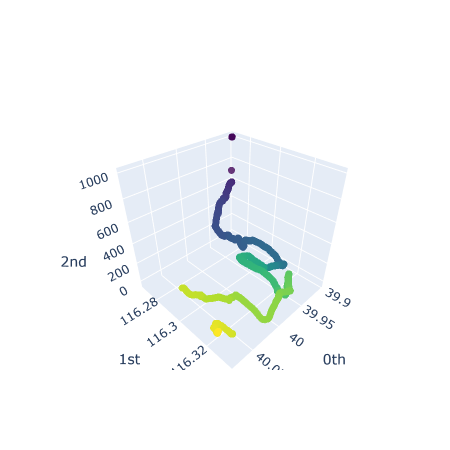
\includegraphics[scale=1]{images/Nube_Puntos.png}
    \caption{Visualización de la Nube de Puntos de las trayectorias de Geolife}
    \label{fig:nube_puntos}
\end{figure}


\vspace{5cm}

\subsection{Cálculo de Homologías Persistentes}

Una vez visualizados los datos, se procede a realizar un análisis utilizando la técnica de homologías persistentes, uno de los pilares fundamentales del análisis topológico de datos. Para la presente implementación, se decidió hacer uso de este método para el cálculo de homologías persistentes de complejos de \textit{Vietoris-Rips}, permitiéndonos extraer información clave sobre las características topológicas de los datos a lo largo de diferentes escalas. Esta implementación se realizó utilizando el módulo \textit{VietorisRipsPersistence} de la librería \textit{giotto-tda}, especificando como argumentos las dimensionales de homología que son de interées en el análisis, siendo en el ejemplo que se muestra en la Figura \ref{fig:pers_una} tres:

\begin{figure}[h]
    \centering
    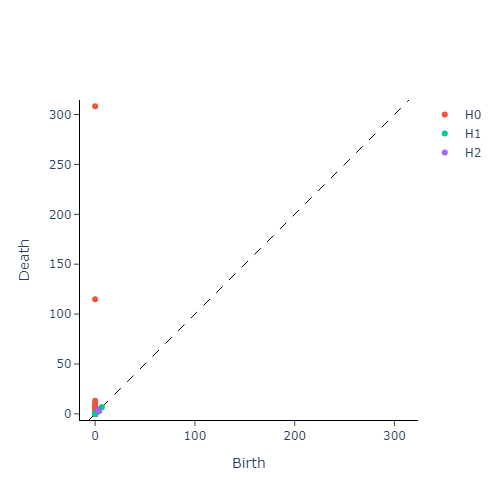
\includegraphics[scale=0.7]{images/persistencia.png}
    \caption{Diagrama de Persistencia de un Conjunto de trayectorias}
    \label{fig:pers}
\end{figure}

Estas tres dimensiones nos permiten observar diferentes estructuras topológicas:

\begin{enumerate}
    \item HO: Nos permite identificar las componentes conexas de la nube de puntos
    \item H1: Nos indica los ciclos presentes en el conjunto de los datos
    \item H2: Nos permite observar las cavidades, o huecos tridimensionales presentes en la estructura
\end{enumerate}

\vspace{2cm}
A la hora de realizar las ejecuciones de esta función, al usar volúmenes de datos de gran dimensiones, los tiempos de ejecución en la misma eran bastantes elevados, con un alto coste computacional, por tanto, se hizo usó de la integración de la librería \textit{giotto-tda} con paralelismo \textit{multi-thread} para agilizar estos procesos de cálculo y generación de gráficas, mejorando los tiempos de ejecución en alrededor de un 200\% usando 15 hilos ejecutando en una sola máquina. 

\begin{figure}[h]
    \centering
    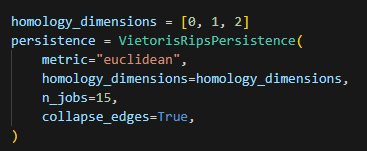
\includegraphics[scale=0.7]{images/codigo_persistencia.png}
    \caption{Definición del objeto VietorisRipsPersistence}
    \label{fig:codigo}
\end{figure}

Una vez hemos definido el objeto \textit{persistence} y realizados los cálculos, se procede a la representación gráfica del diagrama de persistencia, veáse Figura~\ref{fig:pers} . Esta representación se genera haciendo las transformaciones necesarias al objetivo persistencia generando mediante el uso de la función \textit{.fit\_transform}, generando así un objeto para mandar de argumento a la función \textit{plot\_diagram} para generar el diagrama mencionado anteriormente.

\subsection{Extracción de Descriptores con Mapper}

Llegados a este punto, habiendo realizado ya la visualización de los datos y el cálculo de las homologías persistentes, precedemos a la preparación de un pipeline de Mapper, y la representación en forma de grafo de este haciendo uso de las funciones de la librería \textit{giotto-tda}. En primera instancia, es importante dar una breve explicación de en que consiste el algoritmo: "\ Un conjunto de datos $S$, con los siguientes hiperparámetros, tiene asociado el complejo simplicial de Mapper:

\begin{itemize}
    \item Un algoritmo de clusterización y un conjunto de $n$ clústers.
    \item Una función filtro que capture variables latentes a un espacio de dimensión $K$.
    \item Una cubierta abierta de nuestro espacio de variables latentes.
    \item Para cada abierto $U$ del espacio latente y cada $i \leq K$, construimos un conjunto de puntos en $S$ determinado por el $i$-ésimo clúster de la imagen inversa de $U$, es decir, todos los elementos de la base de datos que bajo $f$ van a dar a $U$.
\end{itemize}

La familia de todos los subconjuntos $S(U,i)$ de la base de datos determinada por todas las parejas $(U,i)$ serán los puntos de nuestro complejo simplicial de Mapper. Las caras de este complejo simplicial están determinadas por los subconjuntos que contengan registros de nuestro dataset en común."\   \cite{bourbaki_mapper}

\vspace{5cm}

Teniendo esto en cuenta, procedemos al diseño y configuración del pipeline. Este proceso se compone de los siguientes cuatros pasos:

\begin{itemize}
    \item \textbf{Cartografía} En primer lugar, cartografiamos $D$ a un espacio de menor dimensión usando una función de filtrado de tipo $f: R^n -> R^m$. Se puede elegir de una variedad de funciones para realizar esta tarea, en nuestro análisis decimos hacer uso de una proyección, al darnos la opción la opción de realizar distintos análisis con cambios mínimos en los parámetros del análisis. Todo esto se consigue haciendo uso de la función \textit{FilterFunctionName} de la librería \textit{giotto-tda}, que contiene una gran de variedad de funciones de filtrado, dando libertad al usuario para ajustar el análisis que desea realizar a las características del problema o datos a tratar.  
    \item \textbf{Filtrado} Una vez realizado la proyección, se procede al filtrado de valores de tipo ${\cal U } = (U_i)_ {i\in I}$, para generar un recubrimiento de un conjunto de intervalos que se solapan, con una longitud constante.En esta implementación, se hace uso de un recubrimiento de tipo \texttt{CubicalCover} con \texttt{n\_intervals = 10} y \texttt{overlap\_frac = 0.4}, lo que significa que el espacio filtrado se divide en 10 intervalos por dimensión, cada uno con un solapamiento del 40\%. Esta superposición es esencial para capturar estructuras conectadas en regiones vecinas y evitar una fragmentación excesiva del espacio.
    \item \textbf{Clusterización} Para cada conjunto preimagen $f^{-1}(U_i)$ asociado a cada intervalo del recubrimiento, se aplica un algoritmo de agrupamiento con el objetivo de identificar componentes conexas. En nuestro caso, se emplea el algoritmo \texttt{DBSCAN} (Density-Based Spatial Clustering of Applications with Noise), que tiene la ventaja de no requerir especificar el número de clusters y es robusto frente al ruido y las formas arbitrarias de los datos. Esto lo convierte en una opción adecuada para trayectorias geográficas, donde pueden existir regiones de alta densidad intercaladas con trayectorias dispersas o inusuales.

    \item \textbf{Construcción del grafo} Finalmente, se construye un grafo Mapper, en el cual cada nodo representa un cluster obtenido en algún intervalo, y se crea una arista entre dos nodos si comparten al menos un punto de datos (es decir, si sus conjuntos de puntos tienen intersección no vacía). Este grafo sintetiza la estructura topológica del conjunto de datos original, revelando la conectividad global, la presencia de ciclos o componentes separados, y sirve como herramienta de exploración visual y estructural. 
\end{itemize}

Para la visualización del grafo Mapper resultante del proceso descrito anteriormente, se utiliza la función \texttt{plot\_static\_mapper\_graph} de \texttt{giotto-tda}, que genera una representación estática del grafo que puede ser interpretada fácilmente en el contexto de las trayectorias geoespaciales. Adicionalmente, se hace uso nuevamente de la integración de la librería con paralelismo \textit{multi-thread}, para agilizar la ejecución de la creación de los pipelines de Mapper.

A continuación, se puede ver el resultado de ejecutar este proceso, con un pipeline definido de la siguiente manera: una función de proyección sobre los 3 ejes cartesianos, con un recubrimiento cúbico, y un solapamiento de un 30\%:

\begin{figure}
    \centering
    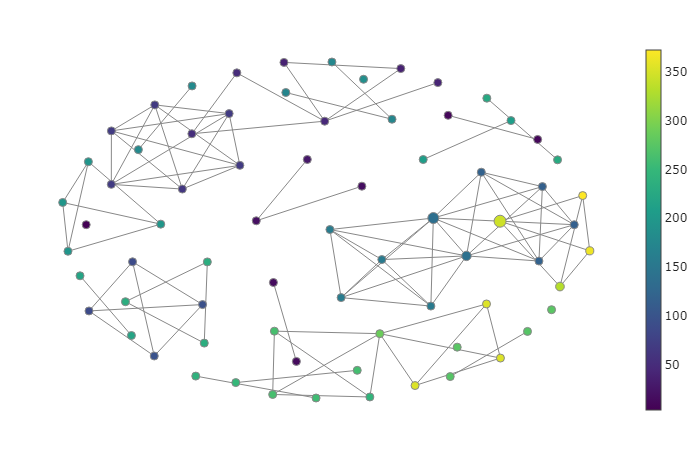
\includegraphics[scale=0.7]{images/mapper.png}
    \caption{Grafo de Mapper generado a partir de una trayectoria del Dataset}
    \label{fig:grafo_mapper}
\end{figure}


\vspace{20cm}
Adicionalmente, para algunas trayectorias en concreto se genero la matriz de distancias haciendo uso de la librería dedicada para Machine Learning de Python, \textit{sklearn}, mas concretamente la funcion \textit{pairwise\_distances}, utilizando la métrica euclidiana, y representando esta gráfica en formato mapa de calor, para visualizar de mejor manera las distancias entre las componentes de la trayectoria.

\subsection{Análisis y comparación con PCA}

Para complementar el análisis topológico y obtener una representación reducida de los datos de trayectoria, se ha empleado la técnica de Análisis de Componentes Principales (PCA). Este método estadístico nos permite proyectar un conjunto de datos multidimensional en un espacio de menor dimensión, conservando la mayor parte de la varianza de los datos originales.

\vspace{0.2cm}

En primer lugar, se ha aplicado PCA sobre la nube de puntos generada anteriormente, cada una de estas trayectorias, inicialmente expresada en coordenadas cartesianas tridimensionales, ha sido transformada mediante PCA a un espacio de dos dimensiones, facilitando de esta manera la visualización de la evolución temporal de los puntos. El resultado se representa mediante un gráfico de dispersión en el que cada punto está coloreado según su componente temporal, permitiendo observar cómo varía la trayectoria a lo largo del tiempo en el nuevo espacio de representación.

\vspace{0.2cm}

A continuación, se ha aplicado también PCA sobre las características extraídas tras aplicar técnicas topológicas, como los diagramas de persistencia y sus correspondientes representaciones vectorizadas. En este caso, la proyección a dos dimensiones permite explorar visualmente si existen agrupaciones o patrones diferenciables en las características topológicas. La visualización se realiza nuevamente como un gráfico de dispersión, donde se espera que trayectorias similares en cuanto a su estructura topológica se agrupen en regiones cercanas del espacio proyectado.

\vspace{0.2cm}

En ambas representaciones, se ha utilizado \texttt{matplotlib} y \texttt{seaborn} para la visualización de los resultados. Estas herramientas permiten no solo visualizar los componentes principales, sino también identificar posibles agrupaciones, transiciones o tendencias que puedan estar ocultas en la representación original de los datos. La comparación entre el espacio proyectado de los datos originales y el espacio proyectado de las características topológicas constituye un recurso valioso para validar y entender las transformaciones realizadas mediante TDA.

\vspace{0.2cm}

Este enfoque no topológico se ha utilizado como una técnica complementaria, tanto para interpretar los datos de entrada como para evaluar la riqueza estructural de los descriptores generados mediante homología persistente, estableciendo así una comparación visual y cuantitativa entre representaciones convencionales y topológicas.

\vspace{2cm}

\section{Técnicas estadísticas para el análisis de trayectorias GPS} A diferencia de los métodos basados en Análisis Topológico de Datos (TDA) \cite{chazal2021introduction} \cite{hensel2021survey}, el enfoque clásico emplea técnicas convencionales de análisis estadístico y de aprendizaje automático. Estas técnicas se utilizan como línea base comparativa, aprovechando la facilidad de interpretación y la robustez de su metodología \cite{refBase1}. A continuación se enumeran de manera breve los pasos principales del pipeline clásico implementado, las herramientas utilizadas y cómo estas metodologías permiten capturar la forma y similitud de las trayectorias usando métricas tradicionales:

\begin{enumerate}
\item \textbf{Preprocesamiento de datos:} se limpian las trayectorias GPS eliminando puntos erróneos o valores atípicos, se corrigen saltos de señal y se muestrean las trayectorias a longitudes uniformes \cite{refPreproc}. Este tratamiento inicial facilita el análisis posterior al homogenizar la representación de cada ruta.
\item \textbf{Extracción de características:} cada trayectoria se convierte en un vector numérico que describe su forma o recorrido. Esto puede lograrse mediante el muestreo regular de coordenadas espaciales (latitud/longitud) o la obtención de estadísticas agregadas (distancia total recorrida, velocidad media, ángulos de cambio de dirección, etc.) \cite{refFeatures}. Estas características resumen las propiedades geométricas y dinámicas de cada trayectoria.
\item \textbf{Reducción de dimensionalidad (PCA):} se aplica Análisis de Componentes Principales (PCA) para proyectar los datos en un espacio de menor dimensión \cite{refPCA}. El PCA identifica las direcciones de máxima varianza en el conjunto de trayectorias y permite conservar las componentes principales (generalmente las primeras 2 o 3), capturando la forma global de las rutas con pocos parámetros \cite{refPCA}.
\item \textbf{Agrupamiento (clustering):} sobre los datos reducidos se ejecutan algoritmos de clustering clásicos. Por ejemplo, K-means agrupa las trayectorias en un número fijo de clústeres, minimizando la varianza interna de cada grupo \cite{refKMeans}. En paralelo, DBSCAN (Density-Based Spatial Clustering) identifica grupos basados en la densidad de puntos en el espacio de características, permitiendo descubrir clústeres de forma arbitraria sin conocer de antemano el número de grupos y diferenciando ruido de datos dispersos \cite{refDBSCAN}. Estas técnicas agrupan trayectorias con formas o patrones similares.
\item \textbf{Cálculo de métricas de similitud:} para cuantificar la similitud entre trayectorias se emplean métricas convencionales. Esto incluye distancias euclídeas o Manhattan entre vectores de características, así como distancias propias de trayectorias (por ejemplo, la distancia de Fréchet o el Dynamic Time Warping (DTW)) \cite{refFrechet} \cite{refDTW}. Estas medidas numéricas permiten evaluar cuán semejantes son las rutas en cuanto a su forma y recorrido, complementando el agrupamiento con una evaluación explícita de la similitud.

\vspace{3cm}

\item \textbf{Visualización de resultados:} finalmente, se utilizan herramientas de visualización para interpretar los resultados. Se emplean bibliotecas de Python como Matplotlib y Seaborn para generar gráficos bidimensionales de las componentes principales y mapas de calor \cite{refMatplotlib} \cite{refSeaborn}. Asimismo, es posible trazar directamente las rutas GPS en un plano geográfico, coloreando cada trayectoria según el clúster asignado. Estas visualizaciones facilitan la inspección visual de patrones de movilidad y la comparación con los patrones obtenidos mediante TDA.
\end{enumerate} Los métodos descritos capturan la forma de las trayectorias mediante su representación numérica y evalúan la similitud a través de métricas clásicas de distancia. Aunque este enfoque clásico no explora explícitamente la estructura topológica de los datos, proporciona una base sólida y comprensible que puede compararse con los resultados del análisis topológico \cite{refComparison}. En conjunto, las técnicas de PCA y clustering tradicionales permiten obtener patrones globales en los datos de movilidad y sirven como complemento para evaluar las ventajas del enfoque topológico.
% Secciones creadas por alumno
\chapter{Resultados de TDA sobre trayectorias} \label{chp:resultados}
En este capítulo se presentan los resultados obtenidos a lo largo del análisis topológico de trayectorias utilizando técnicas de TDA, junto con algunos enfoques comparativos mediante métodos clásicos de análisis de datos. El objetivo principal de esta sección es mostrar de forma clara y estructurada cómo las herramientas aplicadas permiten extraer información significativa sobre la estructura de los datos, tanto a nivel local como global.

\vspace{0.2cm}

Se incluyen visualizaciones de nubes de puntos generadas a partir de trayectorias GPS del conjunto Geolife, así como sus correspondientes diagramas de persistencia, representaciones PCA y grafos Mapper. También se analizan las propiedades topológicas identificadas —como ciclos persistentes o conectividad— y se discuten sus implicaciones. Adicionalmente, se presentan resultados de métodos alternativos no topológicos (como clustering y reducción de dimensionalidad) con el fin de establecer una comparación cualitativa entre enfoques.

\vspace{0.2cm}

La interpretación de los resultados se centra tanto en trayectorias individuales como en el comportamiento agregado del conjunto de datos, permitiendo evaluar la capacidad del TDA para detectar patrones globales, anomalías y propiedades invariantes que no son fácilmente identificables mediante técnicas convencionales.


\section{Resultados} \label{sct:resultados_resultados}

Durante este capítulo, se van a plantear los resultados del análisis topológico de datos explicada a lo largo del capítulo \ref{chp:desarrollo} sobre una sola trayectoria del dataset \textit{Geolife}, sobre un conjunto de trayectorias consecutiva del mismo, y sobre otro conjunto de trayectorias no relacionadas entre sí, así como la aplicación de estos mismos datos en su contraparte implementada con métodos tradicionales. Posteriormente, se presentarán las características topológicas observadas a lo largo del desarrollo, y se hará una breve comparativa entre las 2 soluciones, y se intentará dar una visión a las diferencias entre los resultados en la ejecución de las mismas.

\vspace{2cm}
En primer lugar, vamos a observar el resultado de aplicar estos análisis a una sola trayectoria del conjunto \textit{Geolife}. Como se ha visto anteriormente en el capítulo \ref{chp:desarrollo}, en primer lugar se realizó una visualización de mapa de puntos en 3 dimensiones de la trayectoria en sí. 

Se observa en este caso que al ser una trayectoria de puntos consecutivos, se ve una linea bien definida en su movimiento, pudiendo deducirse que produjo un desplazamiento mayormente vertical en primera, seguido de una serie de desplazamientos horizontales que podrían asimilar la toma de una curva.

\begin{figure}[H]
    \centering
    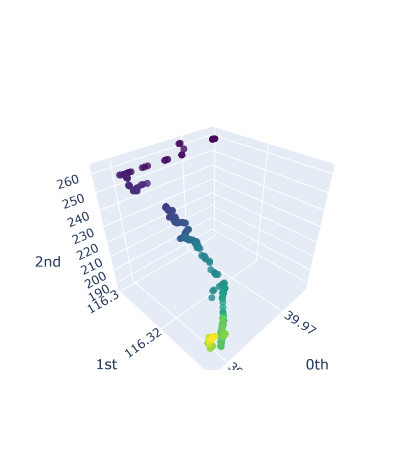
\includegraphics[scale=0.5]{images/puntos_trayec_sola.png}
    \caption{Nube de puntos de una Trayectoria}
    \label{fig:sola_trayec_nube}
\end{figure}

Esta visualización nos ofrece una primera idea de las características topológicas que podría tener esta trayectoria. En general, la visualización 3D no es eficaz, al ser compleja, y no es compatible con trayectorias de mayor dimensión. Para poder obtener resultados, debemos aplicar las herramientas mencionadas anteriormente, como seria la generación del diagrama de persistencia \ref{fig:pers_una} y el grafo Mapper \ref{fig:grafo_mapper}, así como la matriz de distancia entre los puntos de la trayectoria \ref{fig:matriz}. 

\begin{figure}[htbp]
    \centering
    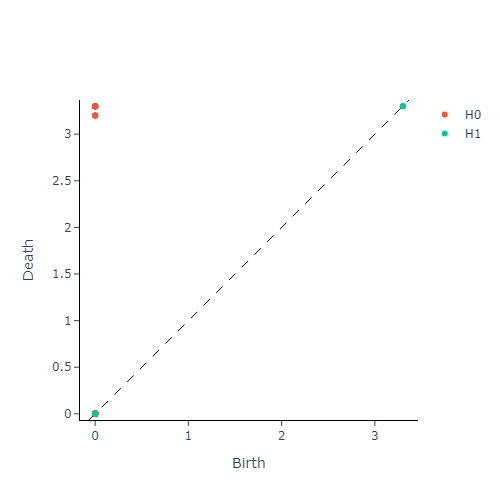
\includegraphics[width=0.7\linewidth]{images/persistencia_una.png}
    \caption{Diagrama de Persistencia de una trayectoria }
    \label{fig:pers_una}
\end{figure}

\begin{figure}[htbp]
    \centering
    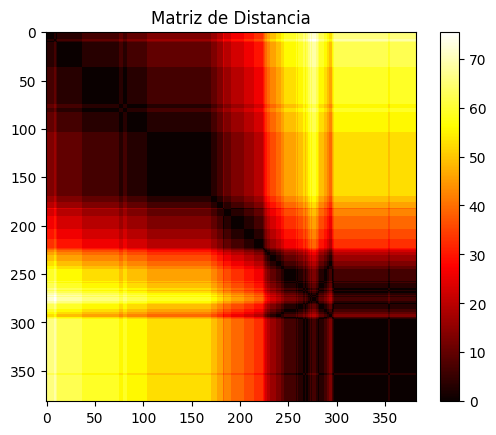
\includegraphics[scale=0.75]{images/matriz.png}
    \caption{Matriz de Distancia de los puntos de la trayectoria}
    \label{fig:matriz}
\end{figure}

\begin{figure}[htbp]
    \centering
    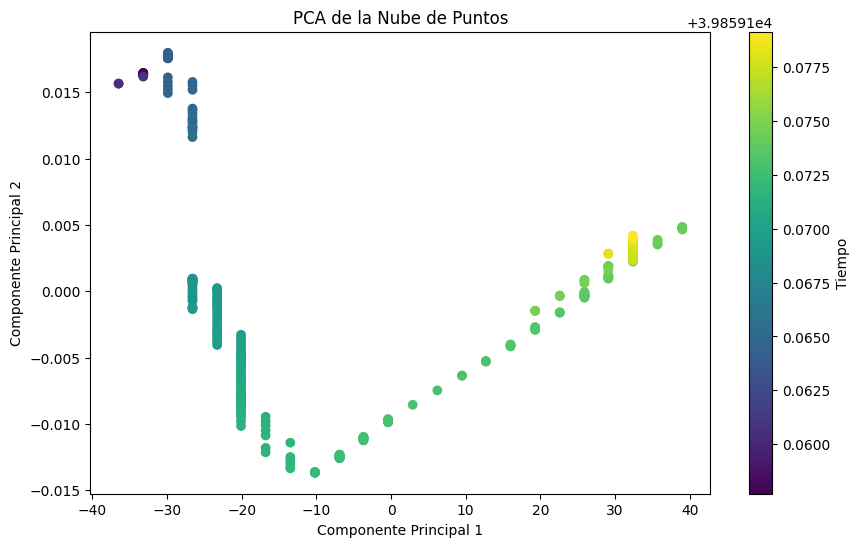
\includegraphics[width=0.75\linewidth]{images/pca_una.png}
    \caption{Análisis con PCA}
    \label{fig:enter-label}
\end{figure}

A partir de estos tres componentes del análisis, podemos afirmar una serie de hechos sobre la naturaleza de esta trayectoria. En primer lugar, 
la visualización en tres dimensiones ( Figura \ref{fig:sola_trayec_nube} ) nos indica que la trayectoria es continua en el espacio, sin cambios abruptos en altitud ni desplazamientos bruscos en el plano horizontal. Este comportamiento sugiere que el movimiento del agente fue progresivo y suave, lo que es coherente con trayectorias humanas o de vehículos en contextos urbanos o semiurbanos.

En segundo lugar, el análisis topológico de la trayectoria mediante homología persistente (Figura~\ref{fig:pers_una}) confirma que la trayectoria se comporta como una única componente conexa (grupo de homología \(H_0\)), ya que todos los puntos rojos aparecen cerca del origen y mueren rápidamente. Esto indica que no hay trayectos desconectados ni segmentos aislados dentro del recorrido.

Por otro lado, la presencia de un ciclo detectado en la dimensión uno (\(H_1\)), representado por un punto verde alejado de la diagonal, revela una característica topológica significativa: la trayectoria contiene una curva cerrada o un bucle. Esta información sería difícil de detectar a simple vista, y gracias al enfoque topológico, puede interpretarse como una posible zona de retorno, giro o patrón de navegación circular realizado por el agente.

Finalmente, la ausencia de características en dimensión dos (\(H_2\)) corrobora que no existen cavidades tridimensionales cerradas dentro del conjunto de puntos, lo cual es esperable dado que el movimiento ocurre sobre una superficie terrestre y no en un volumen tridimensional cerrado.

Además del análisis topológico, se aplicó una reducción de dimensionalidad utilizando Análisis de Componentes Principales (PCA) con el objetivo de visualizar la trayectoria en un espacio bidimensional conservando la mayor varianza posible de los datos originales. En este análisis, se observó cómo la trayectoria proyectada mantiene una estructura coherente, lo que valida que la geometría global del recorrido puede conservarse parcialmente incluso al reducir la dimensionalidad. No obstante, a diferencia del análisis topológico, el PCA no es capaz de identificar la presencia de bucles o estructuras conexas, ya que estas propiedades no se manifiestan directamente en la varianza lineal de los datos.

En este apartado, vamos a observar el resultado de aplicar herramientas topológicas a un \textbf{conjunto de trayectorias}, utilizando el framework desarrollado y descrito en el capítulo \ref{chp:desarrollo}. Para ello, se aplicaron técnicas de Análisis Topológico de Datos (TDA), comenzando con la construcción del grafo Mapper, el cálculo de la homología persistente y la proyección mediante Análisis de Componentes Principales (PCA).

\begin{figure}[htbp]
    \centering
    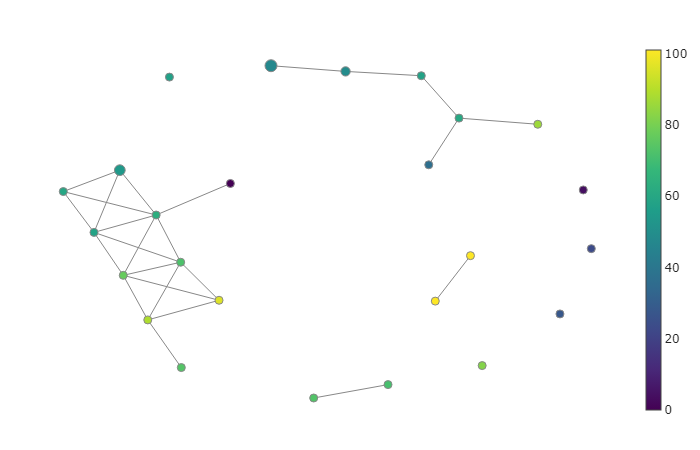
\includegraphics[width=0.75\linewidth]{images/MAPPER_VARIAS.PNG}
    \caption{Grafo Mapper de múltiples trayectorias}
    \label{fig:grafo_mapper_varias}
\end{figure}

En la Figura \ref{fig:grafo_mapper_varias}, se presenta el resultado del algoritmo Mapper aplicado al conjunto completo. Esta visualización revela una estructura compuesta por varias componentes conectadas y otras aisladas. Se puede observar una componente densa (a la izquierda del grafo), que agrupa trayectorias con características similares, mientras que otros nodos aislados indican trayectorias con comportamientos significativamente distintos. La coloración de los nodos representa algún valor escalar asignado, como una función de filtro (por ejemplo, centralidad o densidad), lo que permite identificar posibles agrupamientos o trayectorias atípicas.

\begin{figure}[htbp]
    \centering
    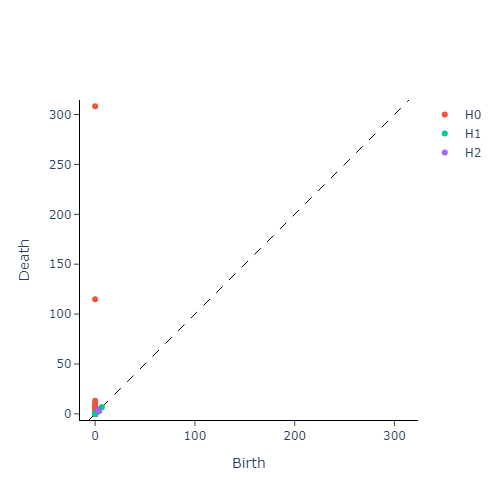
\includegraphics[width=0.7\linewidth]{images/persistencia.png}
    \caption{Diagrama de Persistencia para el conjunto de trayectorias}
    \label{fig:pers_varias}
\end{figure}

La Figura \ref{fig:pers_varias} muestra el diagrama de persistencia del conjunto, el cual permite analizar las características topológicas de las trayectorias en distintas dimensiones. En el módulo de homología cero ($H_0$), correspondiente a componentes conexas, observamos un gran número de puntos que nacen y mueren rápidamente, lo cual sugiere que muchas trayectorias comienzan como componentes aisladas que se conectan gradualmente. Algunos puntos rojos más lejanos de la diagonal indican componentes que persisten más tiempo, es decir, trayectorias bien definidas y separadas del resto.

En el módulo de homología ($H_1$), representada por los puntos verdes, se observa la presencia de varios ciclos, algunos de los cuales son persistentes. Esto indica que dentro del conjunto existen trayectorias que forman bucles o retornos. Estas estructuras topológicas son relevantes, ya que pueden estar relacionadas con patrones de desplazamiento cíclico, como recorridos circulares, vueltas o trayectorias repetitivas en ciertos espacios.

Se detecta un solitario punto en módulo de homología ($H_2$), siendo este punto una anomalía entre los valores de las trayectorias, posiblemente un error a la hora de medir los datos en alguno de los instantes tomados, ya que al representar las trayectorias movimientos sobre superficies planas o cuasi-planas (como mapas urbanos) y no en espacios tridimensionales cerrados, no debería haber cavidades dentro de este conjunto consecutivo de trayectorias. Al revisar los datos, se observa que efectivamente un error en los valores de una de las 110 trayectorias leídas es el causante de este punto. Este valor habría sido casi imposible de detectar sin hacer uso de este tipo de métodos.

\begin{figure}[htbp]
    \centering
    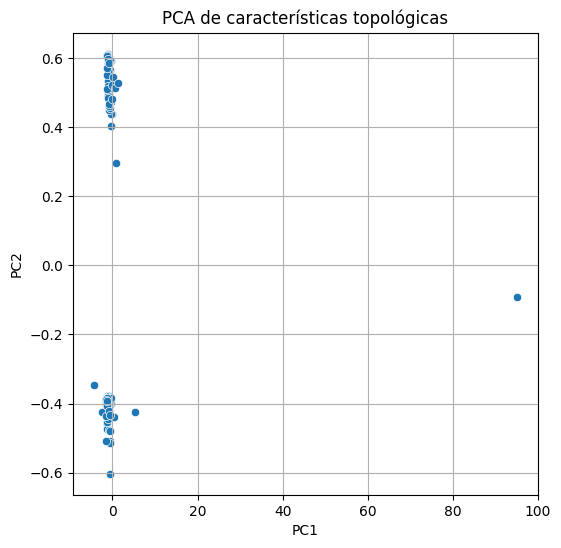
\includegraphics[width=0.75\linewidth]{images/pca_varias.png}
    \caption{Análisis PCA de características topológicas}
    \label{fig:pca_varias}
\end{figure}

En la Figura \ref{fig:pca_varias}, se presenta la proyección de las trayectorias en un espacio de dos dimensiones mediante PCA. Esta técnica se aplicó a los vectores de características topológicas derivados (como la persistencia en $H_0$, $H_1$, entre otros). La mayoría de los puntos se agrupan en una región cercana al eje vertical, lo cual indica que comparten una estructura topológica similar. Sin embargo, destaca un punto que se aleja notablemente en el eje $PC1$, lo que sugiere la presencia de una trayectoria con una topología significativamente diferente al resto. Esta trayectoria podría corresponder a un \textit{outlier}, detectado gracias al poder de discriminación del análisis topológico.

\vspace{0.4cm}

En conjunto, estos tres componentes del análisis nos permiten concluir que el conjunto de trayectorias analizado presenta una variedad rica de estructuras topológicas. Existen trayectorias que forman patrones recurrentes (loops), algunas con comportamiento similar agrupadas en clústeres, y otras más atípicas o anómalas. Herramientas como Mapper, homología persistente y PCA permiten explorar estos datos más allá de su geometría directa, capturando propiedades de conectividad, ciclos y diversidad estructural.

\subsection{Análisis de clustering y comparación con métodos de TDA}

Además del análisis topológico previamente presentado, se exploraron otros métodos más tradicionales para el análisis de las trayectorias, con el fin de contrastar sus resultados y comprender mejor la naturaleza del conjunto de datos. Para ello, se aplicaron técnicas de agrupamiento como DBSCAN y KMeans, así como un Análisis de Componentes Principales (PCA) clásico sobre todas las trayectorias reducidas. 

En primer lugar, en la Figura~\ref{fig:tsne_cluster} se presentan los resultados de la reducción de dimensionalidad mediante t-SNE, sobre la cual se aplicaron los algoritmos de agrupamiento DBSCAN y KMeans.

\begin{figure}[htbp]
    \centering
    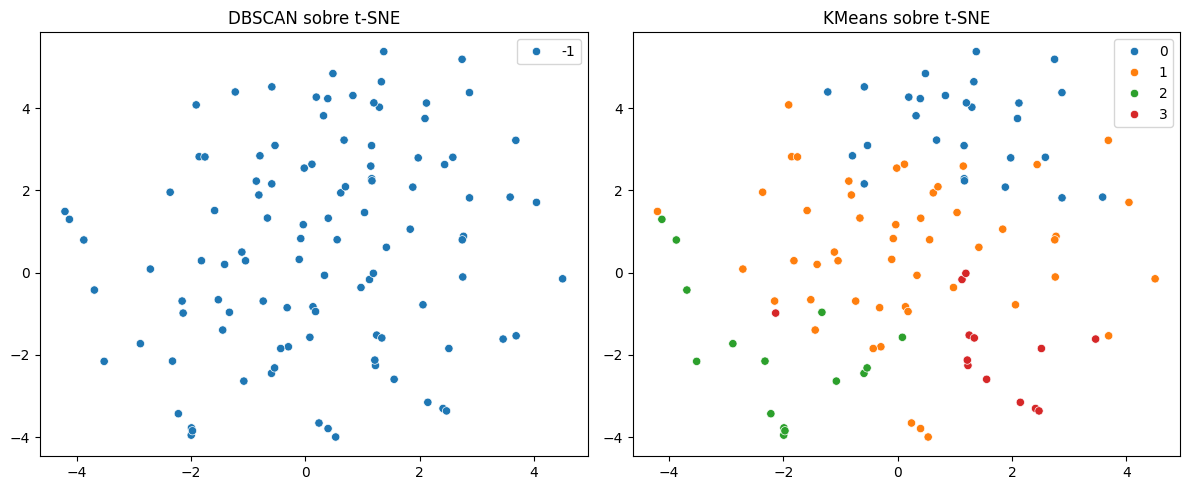
\includegraphics[width=\linewidth]{images/dbscan_kmeans.png}
    \caption{Resultados de clustering sobre reducción t-SNE: DBSCAN (izquierda) y KMeans (derecha)}
    \label{fig:tsne_cluster}
\end{figure}

En el caso de DBSCAN, se observa que el algoritmo no logra identificar estructuras claras de agrupamiento, asignando a todos los puntos la misma etiqueta (o marcándolos como ruido). Esto sugiere que las trayectorias no presentan densidades locales suficientemente diferenciadas para que DBSCAN pueda formar clústeres robustos, o que los parámetros utilizados no eran adecuados para la distribución de los datos en este espacio reducido. Este comportamiento contrasta con los resultados del análisis topológico, donde se identificaban componentes conectadas y ciclos, lo cual indica que sí existe una estructura no trivial en los datos que DBSCAN no ha podido capturar.

Por otro lado, el método KMeans sí fue capaz de dividir el conjunto en cuatro clústeres distintos. Estos grupos parecen estar distribuidos con cierta coherencia espacial, aunque el método se basa únicamente en distancias euclidianas en el espacio reducido por t-SNE. Sin embargo, KMeans no puede detectar bucles o estructuras de conectividad, lo cual representa una limitación frente al análisis de homología persistente. A pesar de ello, los resultados de KMeans pueden ser útiles para la clasificación general de patrones de trayectorias en función de su forma proyectada.

También se realizó un Análisis de Componentes Principales (PCA) tradicional sobre el conjunto de trayectorias para visualizar la distribución global de las mismas en un espacio linealmente reducido (Figura~\ref{fig:pca_tradicional}).

\begin{figure}[htbp]
    \centering
    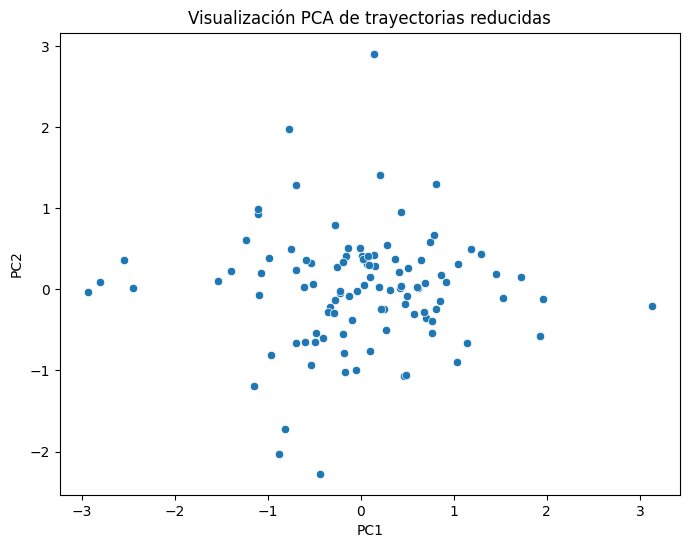
\includegraphics[width=0.75\linewidth]{images/PCA_tradicional.png}
    \caption{PCA tradicional sobre trayectorias}
    \label{fig:pca_tradicional}
\end{figure}

En esta representación, se aprecia una nube de puntos concentrada cerca del origen, con algunas trayectorias dispersas hacia los extremos. Esto indica una cierta homogeneidad en el comportamiento general de las trayectorias, con algunas excepciones que podrían representar trayectos atípicos. No obstante, al igual que en el PCA aplicado a características topológicas, esta visualización no permite identificar características como ciclos o componentes desconectadas, las cuales son evidenciadas únicamente a través del análisis topológico.

\bigskip

\textbf{Comparación con métodos topológicos:}

\begin{itemize}
    \item \textbf{PCA y t-SNE:} Ambos métodos de reducción de dimensionalidad son útiles para representar visualmente la distribución de trayectorias, pero no capturan propiedades topológicas como la conectividad o la existencia de ciclos. Esto limita su capacidad para detectar patrones más complejos de movimiento.
    
    \item \textbf{DBSCAN y KMeans:} Estos algoritmos permiten segmentar los datos en grupos, pero dependen fuertemente de la métrica y del espacio de representación. En especial, DBSCAN no resultó efectivo en este contexto. KMeans, aunque más útil, tampoco proporciona información sobre la estructura topológica de las trayectorias.
    \item \textbf{Homología Persistente y Mapper:} En comparación, el análisis topológico ofrece una visión más rica del comportamiento de las trayectorias. Permite detectar bucles, componentes conexas y variaciones estructurales que los métodos convencionales no logran identificar.
\end{itemize}

En conclusión, los métodos clásicos como PCA, t-SNE y clustering son complementarios al análisis topológico. Mientras los primeros proporcionan una visión global basada en distancias y varianza, el segundo aporta información clave sobre la forma y conectividad de las trayectorias, siendo particularmente útil para identificar patrones complejos de movimiento.



%%%%%%%%%%%%%%%%%%%%%%%%%%%%%%%%%%%%%%%%%%%%%%%%%%%%%%%%%%%%%%%%%%%%%%%%%%%%%%%%
%%%%%%%%%%%%%%%%%%%%%%%%%%%%%%%%%%%%%%%%%%%%%%%%%%%%%%%%%%%%%%%%%%%%%%%%%%%%%%%%










\chapter{Conclusiones} \label{chp:impacto}

%%%%%%%%%%%%%%%%%%%%%%%%%%%%%%%%%%%%%%%%%%%%%%%%%%%%%%%%%%%%%%%%%%%%%%%%%%%%%%%%
%%%%%%%%%%%%%%%%%%%%%%%%%%%%%%%%%%%%%%%%%%%%%%%%%%%%%%%%%%%%%%%%%%%%%%%%%%%%%%%%

\section{Evaluación de objetivos}

La presente sección tiene como finalidad valorar el grado de cumplimiento de los objetivos definidos al inicio de este Trabajo Fin de Grado. El objetivo general consistía en desarrollar una metodología integral para el análisis topológico y estadístico de trayectorias en espacios de baja y alta dimensión, permitiendo extraer información relevante para su interpretación y clasificación. Para lograrlo, se establecieron una serie de objetivos específicos que han guiado el desarrollo del proyecto y que, en su conjunto, han sido abordados satisfactoriamente.

En primer lugar, se ha llevado a cabo una correcta definición y documentación del problema, delimitando las variables relevantes para el estudio de trayectorias en contextos tanto físicos como abstractos. Esta tarea incluyó la selección del conjunto de datos (GeoLife), la identificación de los atributos espaciales y temporales clave y la representación de las trayectorias en forma de nubes de puntos tridimensionales, preparadas para su análisis mediante herramientas topológicas.

A continuación, se diseñó una metodología de análisis que integró con éxito técnicas de Análisis Topológico de Datos (TDA) como la homología persistente y el algoritmo Mapper, junto con métodos estadísticos tradicionales y algoritmos de agrupamiento. Este diseño metodológico permitió identificar patrones estructurales en los datos, tales como bucles, componentes conexas y trayectorias atípicas, aportando una perspectiva más rica que la proporcionada por enfoques puramente estadísticos.

La implementación de la propuesta se realizó utilizando un conjunto de herramientas en el lenguaje Python, incluyendo librerías especializadas como Giotto-TDA, Scikit-learn y Pandas. Esta implementación fue puesta a prueba mediante diversos experimentos que validaron la eficacia de la metodología propuesta. Se evaluaron aspectos como la robustez frente al ruido, la sensibilidad ante anomalías y la eficiencia computacional, especialmente al aplicar técnicas de paralelización para mejorar los tiempos de ejecución.

Finalmente, los resultados fueron interpretados y sintetizados de forma rigurosa. Se analizaron las estructuras topológicas detectadas en los datos, se compararon con los resultados obtenidos por métodos tradicionales como PCA y clustering, y se discutieron las implicaciones prácticas del enfoque propuesto. 

Esta evaluación permitió extraer conclusiones relevantes para el campo del análisis de trayectorias, destacando las ventajas del uso de TDA frente a técnicas convencionales y proponiendo líneas futuras de investigación orientadas a su integración con modelos de aprendizaje profundo.

En resumen, los objetivos planteados en este trabajo han sido cumplidos de manera sólida, evidenciando la utilidad del enfoque topológico-estadístico en el análisis de trayectorias y demostrando su potencial para aplicaciones en movilidad, sistemas dinámicos y análisis de datos complejos.


\section{Trabajo futuro} \label{sct:resultados_trabajofuturo}

Este proyecto nos ofrece una visión relativamente limitada de la potencia que poseen las herramientas de análisis especificas para TDA, al no tener a disposición ni el tiempo ni los recursos computacionales que harian falta para una investigación más en detalle. Se podrían abrir varias líneas de investigaciones relativas a una variedad de factores, ya sea los factores relativos al uso de recursos computacionales, aquellos relativos a los datos usados, etc.

En primer lugar, desde el punto de vista de la mayor explotación de la potencia de las herramientas de análisis, se plantearía el uso de otras herramientas o librerías especificas de TDA, ya sea haciendo uso de otras funciones disponibles dentro de la propia librería \textit{giotto-tda}, o haciendo uso de alternativas como las mencionadas en la sección \ref{Herramientas} del capítulo de estado del arte. Adicionalmente, se podría hacer uso de volúmenes de datos mayores, aprovechando la capacidad de integración de la librerías de análisis con multi-threading, ya sea haciendo uso de recursos computacionales para alto rendimiento en servicios en la nube, o solicitando el uso de súper computadores como podría ser el Magerit-3.

En segundo lugar, el proyecto se podría expandir modificando los datos que son objetos del análisis, ya que el uso de otro tipo de trayectorias físicas o del mundo real, como podría ser el uso de datos médicos, o plantear alternativas basadas en fenómenos más abstractos, como podrían ser los atractores caóticos o espacios fuera de métricas tradicionales como sería la euclidiana, podrían abrir líneas de desarrollo que podrían generar bastante interés. 

Partiendo de la idea de modificar los datos, se podrían hace ligeras transformaciones a las trayectorias usadas actualmente para ver la evolución de las características topológicas de las mismas, por ejemplo, aplicando desplzamientos, o lag, en ciertos intervalos de los datos, generando conjuntos de datos de mayor dimensionalidad, que revelan la depedencia espacial y temporal, y la oportunidad de analizar no solamente la naturaleza de los datos, sino también su robustez ante estos cambios.

Finalmente, se podría expandir el proyecto haciendo uso de soluciones híbridas, implementando las herramientas de clusterizacion y análisis habitualmente usadas en machine learning y análisis de datos, y combinándolas con las soluciones de TDA para poder un análisis mas completo, que nos ofrece una visión más global de las características de un determinado conjunto de datos.

\section{Conclusiones personales} \label{sct:resultados_conclusiones}

La realización de este Trabajo de Fin de Grado ha supuesto un hito de gran valor, tanto en lo académico como en lo personal. Durante el proceso de realización del mismo, he tenido la oportunidad de adentrarme en el campo del Análisis Topológico de Datos (TDA), una disciplina que, si bien requiere de una base matemática sólida para entender algunos de los conceptos clave de la misma, con conocimientos básicos de programación, se nos ofrece un conjunto de herramientas muy potentes para el estudio de estructuras de datos no triviales, como lo son las trayectorias espaciales, que nos permiten realizar análisis de una complejidad considerable, ofreciéndonos una alternativa más optimizada respecto las que nos darían los métodos de análisis tradicional.

A lo hora de ejecutar con una sola trayectoria, se seleccionó una trayectoria de complejidad media, de alrededor de 90 puntos, todos en intervalos de tiempo consecutivos

En lo relativo a los conocimientos técnicos, este proyecto me ha permitido consolidar conocimientos en programación científica y herramientas de análisis de datos con Python, especialmente en el uso de bibliotecas especializadas como \texttt{giotto-tda}, \texttt{scikit-learn}, \texttt{matplotlib} y \texttt{pandas}, siendo algunas de estas herramientas de uso común el mercado profesional. También he mejorado mis conocimientos y he ganado experiencia a la hora de manipular conjuntos de datos reales de tamaño considerable (como el dataset de trayectorias \textit{Geolife}), en la depuración de  problemas relacionados con formatos de datasets y limpieza y transformación a conjunto de datos, en la evaluación de necesidad de cómputo y la optimización del rendimiento computacional con herramientas de software, y a gestionar entornos mixtos de desarrollo, tanto en local como en la nube, mediante Google Colab.

Desde el punto de vista metodológico, ha sido muy enriquecedor explorar la comparación entre métodos tradicionales como serian PCA, k-means, DBSC, entre otros, y métodos topológicos, como la homología persistente y el algoritmo Mapper. Esta comparación me ha permitido comprender no solo las ventajas del TDA en cuanto a la robustez frente al ruido o invariancia ante deformaciones suaves, sino también sus limitaciones en términos de complejidad computacional y la necesidad de interpretación de los resultados generados usando estos métodos.

Uno de los mayores retos fue la elección, limpieza y preparación de los datos, al haber una gran variedad de campos que podrían generar análisis de un interés general, y con referencias previas de otras investigaciones, así como la adaptación de las trayectorias a la tecnología usada en el diseño de las soluciones, dada su variabilidad en longitud y estructura. Esto me llevó a diseñar funciones de reducción dimensional adaptativas (como el uso de clustering K-means para homogeneizar longitudes), que posteriormente se integraron dentro de los pipelines de análisis. Asimismo, la visualización de los resultados y la generación de figuras comprensibles fue un aspecto crucial que me ayudó a reforzar mi capacidad de comunicación científica.

En cuanto al impacto personal, considero que este trabajo ha sido una introducción sólida al mundo de la investigación aplicada en ciencia de datos. Me ha motivado a seguir profundizando en campos como el aprendizaje automático basado en geometría y topología, y ha reforzado mi interés por el análisis de patrones espaciales y temporales en entornos reales, como el transporte o la salud. 

Quisiera destacar especialmente la ayuda y orientación que me ha aportado mi tutor, Juan Antonio Fernández del Pozo en todo momento, manteniendo una comunicación fluida y constante, y ofreciéndome información, en forma de documentación, ejemplos, y sugerencias muy valiosas que han ayudado enormemente al resultado de este trabajo, así como la fluidez y constancia en la comunicación, ayudando a mantener unas pautas y un tempo de trabajo constante, que ha ayudado a seguir las tiempos establecidos inicialmente en el plan de trabajo en la medida de lo posible.

Finalmente, valoro positivamente la capacidad que este trabajo me ha aportado a la hora estructurar un proyecto de análisis desde cero, empezando con el planteamiento del problema a resolver, continuando con una planificación de las tareas a realizar en base, y seguido por las diferentes de la realización del mismo, como la revisión extensa de literatura y trabajos previos, desarrollo y experimentación computacional, y síntesis de resultados. Ha sido una experiencia exigente, pero altamente satisfactoria, y considero que me ha preparado tanto para futuros estudios de posgrado como para desafíos profesionales en el ámbito de la analítica avanzada. 

\section{Análisis del Impacto}


\subsection{Impacto general}

El presente trabajo, enfocado en el análisis topológico de trayectorias mediante homología persistente y algoritmos de Mapper con la librería de Python \texttt{Giotto-TDA}, tiene un amplio potencial de aplicación en una multitud de campos. Al extraer características topológicas como componentes conexas, ciclos y cavidades de conjuntos de trayectorias en espacios métricos —por ejemplo, \(\mathbb{R}^2\) para movilidad terrestre o \(\mathbb{R}^3\) para recorridos aéreos o de GPS, este método ofrece descripciones robustas de la estructura global del movimiento. Dichos resúmenes topológicos son invariantes ante deformaciones continuas y resistentes al ruido, lo cual los hace especialmente útiles en escenarios reales donde los datos no estar completos, o no tener la precisión deseada. Como ya se ha mencionado en otras secciones en este mismo documento, este tipo de prácticas tienen especial relevancia en las siguientes áreas:

\begin{itemize}
    \item \textbf{Movilidad urbana:} El análisis topológico de trayectorias permite identificar rutas frecuentes, núcleos de congestión y patrones de movimiento recurrentes. Por ejemplo, ciclos persistentes en diagramas de persistencia pueden corresponder a bucles viales o rutas circulares predominantes. Esta información puede ayudar a optimizar semáforos, carriles exclusivos o zonas peatonales, favoreciendo un desarrollo urbano más eficiente y sostenible.
    
    \item \textbf{Transporte aéreo:} En este contexto, las trayectorias de vuelo se representan como curvas en \(\mathbb{R}^3\) (latitud, longitud, altitud). La homología persistente permite detectar patrones recurrentes, intersecciones o corredores aéreos significativos, mejorando la gestión del tráfico aéreo y la planificación de rutas más eficientes desde el punto de vista energético.
    
    \item \textbf{Sistemas dinámicos:} En contextos matemáticos o físicos, las trayectorias de sistemas dinámicos (como atractores caóticos) muestran estructuras complejas en el espacio de fases. Aplicar homología persistente revela invariantes topológicos que caracterizan el comportamiento del sistema, mientras que el algoritmo Mapper facilita la visualización de estos patrones complejos.
    
    \item \textbf{Otros campos:} Incluyendo logística, análisis ecológico, planificación de robots móviles y salud pública. En todos estos casos, el análisis topológico permite extraer patrones globales de movimiento y detectar trayectorias anómalas con mayor eficacia que los métodos tradicionales.
\end{itemize}

Durante el desarrollo del trabajo se tomaron decisiones metodológicas con el objetivo de maximizar el impacto práctico. Por ejemplo, se empleó la métrica euclidiana en la representación de las trayectorias por su interpretación geométrica intuitiva, y se eligieron funciones de filtro semánticamente relevantes en Mapper (como la distancia recorrida o el tiempo transcurrido). El uso de bibliotecas optimizadas como \texttt{Giotto-TDA} también refuerza la aplicabilidad de los resultados a contextos reales, dada su escalabilidad y compatibilidad con flujos de trabajo de \texttt{machine learning}.

\subsection{Impacto en los Objetivos de Desarrollo Sostenible (ODS)}

El análisis topológico de trayectorias contribuye directa e indirectamente a diversos Objetivos de Desarrollo Sostenible (ODS) definidos en la Agenda 2030:

\begin{figure}[h]
    \centering
    
\includegraphics[scale=0.25]{images/agenda_2030.jpg}
    \caption{Objetivos de Desarrollo Sostenible (ODS) de la Agenda 2030 \cite{ODS}}
    \label{fig:ejemplo}
\end{figure}


\begin{itemize}
    \item \textbf{ODS 11: Ciudades y comunidades sostenibles.} Mejorar la movilidad urbana es fundamental para lograr ciudades más inclusivas, seguras y eficientes. Los métodos propuestos ayudan a reducir la congestión y optimizar las rutas, favoreciendo una planificación urbana basada en datos.

    \item \textbf{ODS 9: Industria, innovación e infraestructura.} El uso de herramientas avanzadas como TDA fomenta la innovación tecnológica en transporte e infraestructura, habilitando nuevos modelos de gestión urbana, control de tráfico o rutas logísticas inteligentes.
    \vspace{2cm}
    \item \textbf{ODS 3: Salud y bienestar.} Una red de movilidad más eficiente contribuye a la salud pública mediante la reducción de accidentes, tiempos de respuesta de emergencias y exposición a la contaminación. Además, el análisis de trayectorias se puede aplicar a estudios epidemiológicos.

    \item \textbf{ODS 13: Acción por el clima.} La optimización de trayectorias y flujos de transporte, ya sea terrestre o aéreo, contribuye a reducir las emisiones de gases de efecto invernadero. Las herramientas desarrolladas pueden emplearse para diseñar rutas de bajo consumo energético.
\end{itemize}

En resumen, aunque este trabajo es principalmente metodológica, sus implicaciones abarcan diversos dominios con relevancia social, científica y ambiental. La capacidad de extraer descripciones topológicas robustas de trayectorias contribuye a la toma de decisiones informadas y sostenibles en múltiples contextos de aplicación.

\printbibliography[heading=bibintoc]

%%-----------------------------------------------
%% Anexos
\appendix
\clearpage
%\addcontentsline{toc}{chapter}{\annexname}
\chapter{Anexo} \label{chp:anexo}

\section{Materiales Desarrollados}
El código, junto con los datos específicos utilizados para generar los resultados para este trabajo se encuentran en https://github.com/krlokbrera/TDA\_CarloCabrera

\section{Uso de Inteligencia Artificial Generativa}

Para la realización de este trabajo, se ha hecho uso de herramientas de IA Generativa, como sería \textit{ChatGPT} \cite{chatgpt_conversacion}, para consultas relativas a la realización de la memoria (estructura de figura en overleaf, generación de citas).

\includegraphics[scale=0.001]{images/anexo.jpg}

\section{Turnitin}

Tanto el informe de originalidad como el recibo digital se encuentran disponibles en el repositorio de Github https://github.com/krlokbrera/TDA\_CarloCabrera , más en concreto en la sección de documentos, junto con los archivos .tex utilizados para generar esta memoria.
%%-----------------------------------------------
\end{document}